\chapter{Fixed Delay Model}

The authors in \cite{gaffmonk}, who studied the LI model, numerically demonstrated the important result that as the fixed time delay is increased, the time taken for patterns to emerge also increases. In this chapter, we first revisit analysis of the LI model through a more careful review of the linear theory presented in \cite{yigaffneyli,jiang}, with the aim of analytically showing a linear dependance between a fixed delay $\tau$ and the time taken for pattern formation, which has not yet been done in the literature, and verify these results through numerical simulations. Through full numerical simulations, we also consider the effects of variations in both initial and boundary conditions on pattern formation.

\section{Linear Analysis}
As defined in \eqref{fixed}, the equations we study for the LI model are
\begin{equation}\label{fixed2}
  \begin{split}
  \frac{\partial u}{\partial t}&=\frac{\epsilon^2}{L^2}\frac{\partial^2u}{\partial x^2}+a-u-2u^2v+3\hat{u}^2\hat{v} \text{ds}\\
  \frac{\partial v}{\partial t}&=\frac{1}{L^2}\frac{\partial^2v}{\partial x^2}+b-u^2v,
\end{split}
\end{equation}
where $u=u(x,t)$, $v=v(x,t)$ and $\hat{u}$, $\hat{v}$ are evaluated at some delay $\tau$, so that $\hat{u}=u(x,t-\tau)$ and $\hat{v}=v(x,t-\tau)$. Following the methodology in \cite{yigaffneyli}, we take a small perturbation about the steady-state $u(x,t)=u_\star+\delta\xi(x,t)$ and $v(x,t)=v_\star+\delta\eta(x,t)$, where $|\delta|\ll 1$. Taylor expanding up to $O(\delta)$ about the steady-state, the linearised dynamics of \eqref{fixed2} are then given by
\begin{equation}\label{linfixed}
  \begin{split}
\frac{\partial\xi}{\partial t}&=\frac{\epsilon^2}{L^2}\frac{\partial^2\xi}{\partial x^2}-\xi-4u_\star v_\star\xi+6u_\star v_\star\hat{\xi}-2u_\star^2\eta+3u_\star^2\hat{\eta},\\
\frac{\partial\eta}{\partial t}&=\frac{1}{L^2}\frac{\partial^2\eta}{\partial x^2}-2u_\star v_\star\xi-u_\star^2\eta,
\end{split}
\end{equation}
with $\hat{\xi}=\xi(x,t-\tau)$ and $\hat{\eta}=\eta(x,t-\tau)$. Substituting into \eqref{linfixed} an ansatz of the form $\begin{pmatrix}\xi\\\eta\end{pmatrix}=\begin{pmatrix}\xi_0e^{-\lambda t}\cos(k\pi x)\\ \eta_0e^{-\lambda t}\cos(k\pi x)\end{pmatrix}$, we obtain the characteristic equation $\mathcal{D}_k=0$, given by,
\begin{equation}\label{characfix}
\mathcal{D}_k=\lambda^2+\alpha_k\lambda+\beta_k+(\gamma_k\lambda+\delta_k)e^{-\lambda\tau}=0,
\end{equation}
where the coefficients are given as,\footnote{We note the coefficient of $\beta_k$ differs from that of \cite{yigaffneyli} due to a suspected error in the cited paper.}
\begin{align}
\alpha_k&=(\frac{\epsilon^2}{L^2}+\frac{1}{L^2})k^2\pi^2+u_\star^2+4u_\star v_\star+1\\
\beta_k&=(\frac{1}{L^2}\pi^2k^2+u_\star^2)(\frac{\epsilon^2}{L^2}\pi^2k^2+4u_\star v_\star+1)-4u_\star^3v_\star\\
\gamma_k&=-6u_\star v_\star\\
\delta_k&=-6\frac{1}{L^2}u_\star v_\star k^2\pi^2.
\end{align}
This characteristic equation can be used to determine the parameter sets $(a,b,\frac{\epsilon^2}{L^2},\frac{1}{L^2},\tau)$ in which a Turing instability occurs, and hence where we expect pattern formation. From \eqref{perturbgrow}, the perturbation grows like $e^{\lambda t}\cos(k\pi x)$, and so if there exists a $k\neq0$ for a given $(a,b,\frac{\epsilon^2}{L^2},\frac{1}{L^2},\tau)$ such that $\Re(\max_k(\lambda))>0$, we expect pattern formation. Figure \ref{fig:dispfixed} shows $\max_k(\Re(\lambda))$ plotted against $\tau$, for multiple given $(a,b)$ parameter sets. The complex roots for $\lambda$ of the characteristic equation were found using the \emph{roots} command of the MATLAB package Chebfun \cite{chebfun}. These plots were produced by varying $k$ over $[0,50]$ at regular discrete intervals of $1$ for a given $\tau$, and for each $k$, the roots of \eqref{realfix} and \eqref{complexfix} were computed. The maximum over the $k$ of the $\Re(\lambda)$ was then taken for $k\in[0,50]$. This was repeated for time delay varied over $\tau\in[0,1]$ at regular intervals of $0.1$. We do not consider a $k$ larger than $50$ as full numerical solutions for the parameter values used tended towards patterns with four `spikes', so we do expect large wave numbers to be excited. All results in this section, unless otherwise stated, were obtained using parameter values $\epsilon^2=0.001$ and $L=30\sqrt{0.05}$

\begin{figure}[H]
    \centering
    \begin{subfigure}[b]{0.45\textwidth}
        \centering
        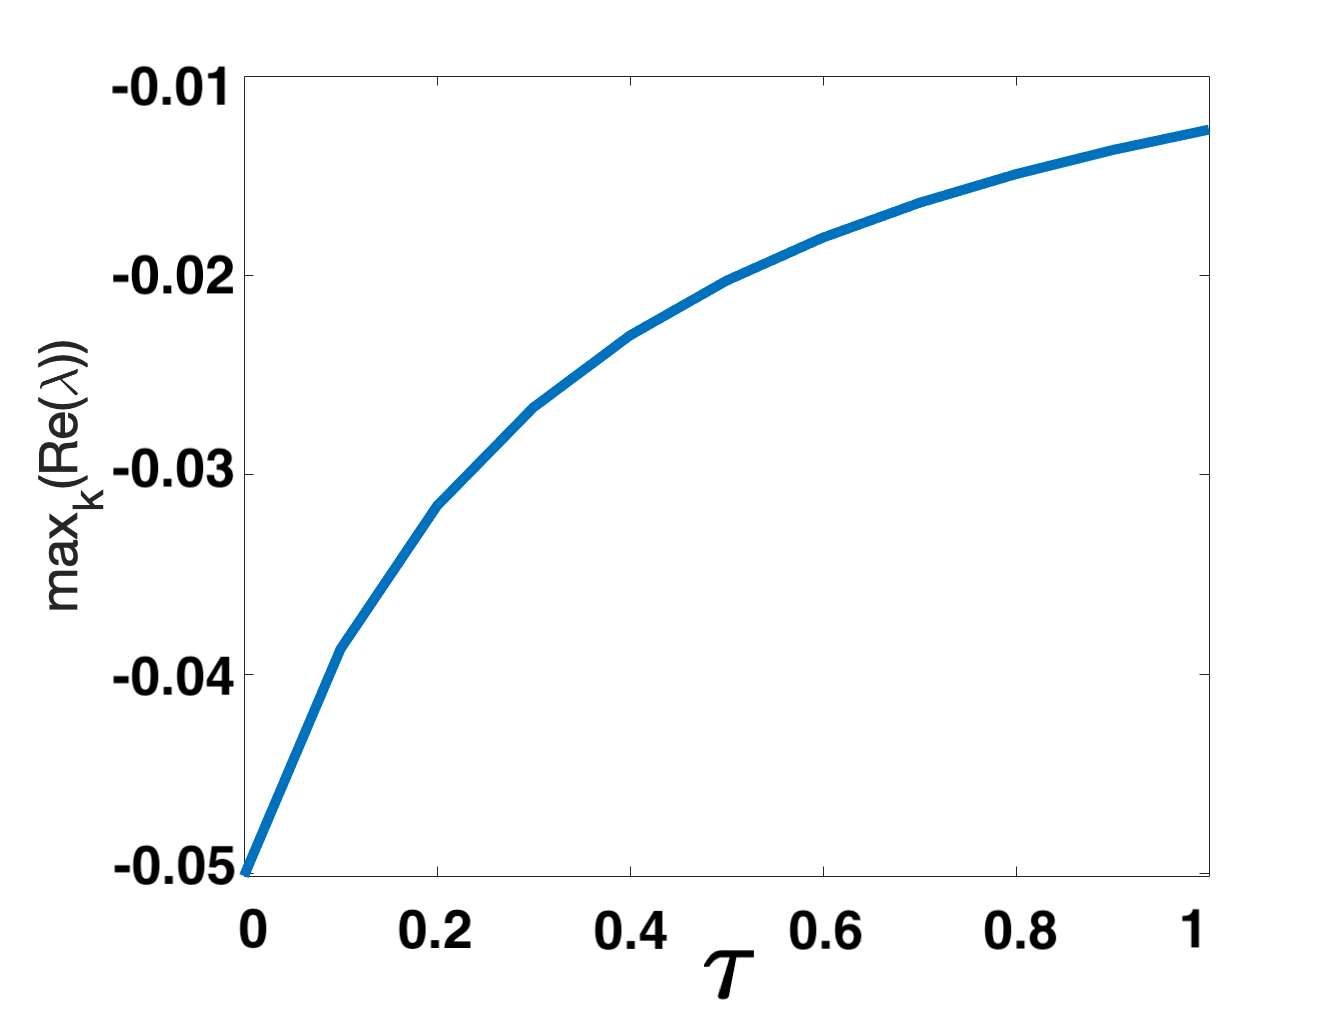
\includegraphics[width=7cm,height = 5.5cm]{disp1.png}
        \caption{$(a,b)=(0.4,0.4)$. $\max_k(\Re(\lambda))<0 \quad \text{for all }\tau\in[0,1]$. Linear theory predicts no pattern formation for all $\tau\in[0,1]$. }
        \label{}
    \end{subfigure}
    \hfill
    \begin{subfigure}[b]{0.45\textwidth}
        \centering
        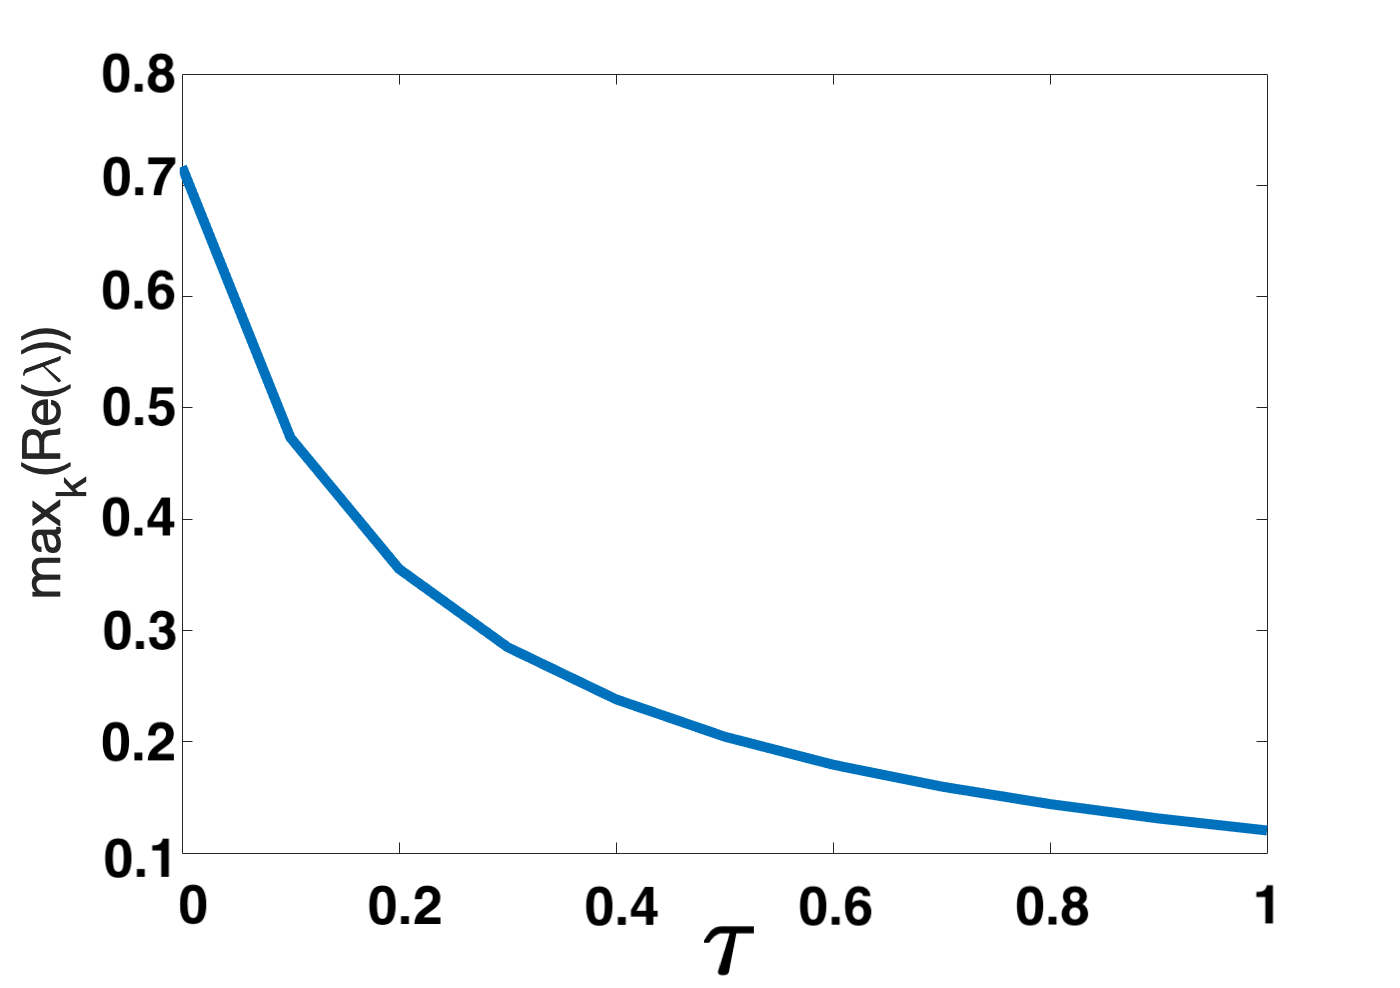
\includegraphics[width=7cm,height = 5.5cm]{disp2.png}
        \caption{$(a,b)=(0.1,0.9)$. $\max_k(\Re(\lambda))>0 \quad \text{for all }\tau\in[0,1]$. Linear theory predicts pattern formation for all $\tau\in[0, 1]$.}
        \label{}
    \end{subfigure}
    \caption{Characteristic equaton \eqref{characfix} solved and $\max_k(\Re{\lambda})$ plotted against $\tau\in[0,1]$ for two different parameter sets. $\epsilon^2=0.001$ and $L=30\sqrt{0.05}$.}
    \label{fig:dispfixed}
\end{figure}
Figure \ref{fig:dispfixed} suggests that for $(a,b)=(0.4,0.4)$ and $\tau\in[0,1]$, no patterns will form. However, we expect to see pattern formation $(a,b)=(0.1,0.9)$. We also hypothesise that since $\max_k(\Re(\lambda))$ at $\tau=0$ is greater than at $\tau=1$, the time taken to pattern formation will be longer at $\tau=1$. This relationship between time-to-pattern and time delay is explored in more detail in section \ref{section:delaypatt}. Numerical results in figures \ref{fig:fixedsim1} and \ref{fig:fixedsim2} verify the findings from figure \ref{fig:dispfixed}, namely that pattern formation does not occur for $(a,b)=(0.4,0.4)$, but does for $(a,b)=(0.1,0.9)$.  This suggests that the linear theory is a good approximation to the full model. We note by convention that the numerical solution of the activator $u$ is plotted.
\begin{figure}[H]
    \centering
    \begin{subfigure}[b]{0.45\textwidth}
        \centering
        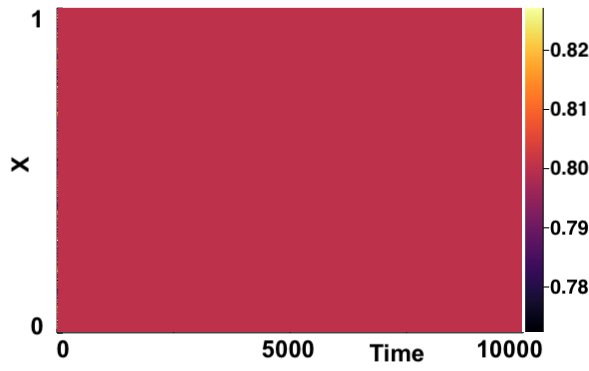
\includegraphics[width=7cm,height = 5.5cm]{nopatt1.png}
        \caption{$(a,b,\tau)=(0.4,0.4,0)$. No pattern formation after $t=10^4$. }
        \label{}
    \end{subfigure}
    \hfill
    \begin{subfigure}[b]{0.45\textwidth}
        \centering
        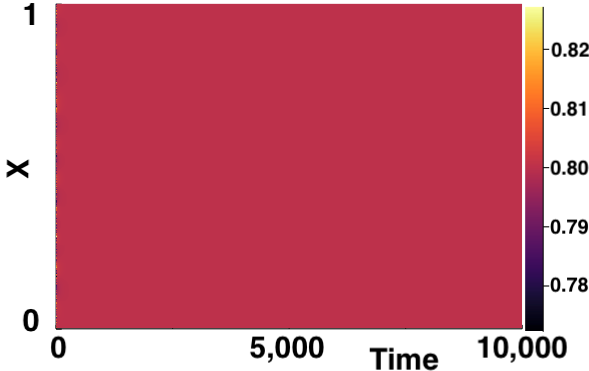
\includegraphics[width=7cm,height = 5.5cm]{nopatt2.png}
        \caption{$(a,b,\tau)=(0.4,0.4,1)$. No pattern formation after $t=10^4$.}
        \label{}
    \end{subfigure}
    \caption{Numerical simulations showing no pattern formation for $(a,b)=(0.4,0.4)$, $\epsilon^2=0.001$ and $L=30\sqrt{0.05}$.}
    \label{fig:fixedsim1}
\end{figure}1

\begin{figure}[H]
    \centering
    \begin{subfigure}[b]{0.45\textwidth}
        \centering
        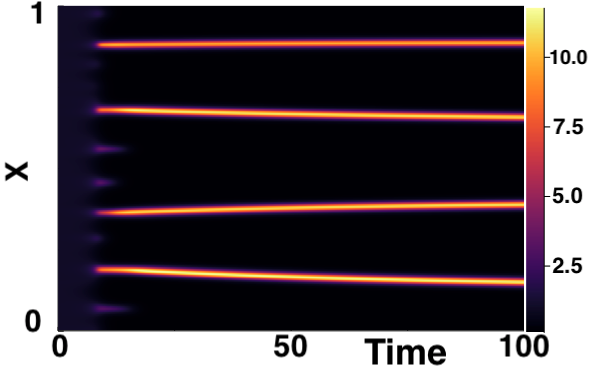
\includegraphics[width=7cm,height = 5.5cm]{patt1.png}
        \caption{$(a,b,\tau)=(0.1,0.9,0)$. Distinct spikes formed at $t\approx7$ }
        \label{}
    \end{subfigure}
    \hfill
    \begin{subfigure}[b]{0.45\textwidth}
        \centering
        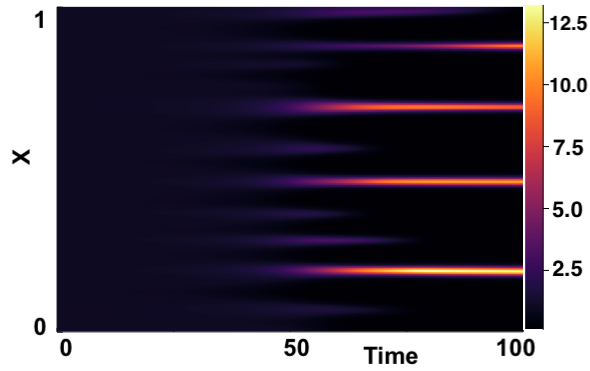
\includegraphics[width=7cm,height = 5.5cm]{patt2.png}
        \caption{$(a,b,\tau)=(0.1,0.9,1)$. Distinct spikes formed at $t\approx50$.}
        \label{}
    \end{subfigure}
    \caption{Numerical simulations showing pattern formation for $(a,b)=(0.1,0.9)$, $\epsilon^2=0.001$ and $L=30\sqrt{0.05}$.}
    \label{fig:fixedsim2}
\end{figure}
These figures were produced using an initial condition $(u_0,v_0)$ given as a random Gaussian perturbation from the homogeneous steady-state. Namely, $$\begin{pmatrix}u_0\\v_0\end{pmatrix}=\begin{pmatrix}u_\star(1+r)\\v_\star(1+r)\end{pmatrix}$$ where $r$ is a random variable such that $r\sim\mathcal{N}(0,0.01)$. The notation $r\sim\mathcal{N}(\mu,\sigma^2)$ denotes a Normally distributed random variable $r$ with mean $\mu$ and standard deviation $\sigma$. A constant history function equal to the initial conditions was used.
\subsection{Bifurcation Analysis}\label{section:fixedbif}
The Turing plot produced in figure \ref{fig:turingspace}, computed using the conditions in \eqref{cond1} and \eqref{cond2}, is a bifurcation diagram indicating regions of Turing instability. We note two separate curves which separate the parameter space into its distinct regions. These will be referred to as the `lines of stability'.
These two curves are indicated in figure \ref{fig:bif0}. The inner arc corresponds to the $(a,b)$ such that $\Re(\lambda)=0$ for the
spatially homogeneous characteristic equation $\mathcal{D}_k$, namely when $k=0$. For $\tau=0$, this corresponds exactly to equating conditions $\eqref{cond1}$ to 0. The outer boundary is the points $(a,b)$ such that $\max_k\Re(\lambda)=0$ for the spatially inhomogeneous characteristic equation $\mathcal{D}_k$. For $\tau=0$, this is identical to equating to the conditions $\eqref{cond2}$ to 0. We split the characteristic equation $\mathcal{D}_k=0$ into its real and imaginary parts, $\mathcal{D}_k^{\Re}=0$ and $\mathcal{D}_k^{\Im}=0$, given by
\begin{align}\label{realfix}
\mathcal{D}_k^{\Re}&=x^2-y^2+\alpha_kx+\beta_k+e^{-x\tau}[\gamma_kx\cos(-y\tau)-\gamma_ky\sin(-y\tau)+\delta_k\cos(-y\tau)]=0,\\
\mathcal{D}_k^{\Im}&=2xy+\alpha_ky+e^{-x\tau}[\gamma_kx\sin(-y\tau)+\gamma_ky\cos(-y\tau)+\delta_k\sin(-y\tau)]=0.\label{complexfix}
\end{align}
By setting $\Re(\lambda)=0$ in equations \eqref{realfix} and \eqref{complexfix}, the real and imaginary parts of $\mathcal{D}_k$ can be simplified to
\begin{align}\label{realfixbif}
  \mathcal{D}_k^{\Re}&=-y^2\beta_k+[-\gamma_ky\sin(-y\tau)+\delta_k\cos(-y\tau)],\\
  \mathcal{D}_k^{\Im}&=\alpha_ky+[\gamma_ky\cos(-y\tau)+\delta_k\sin(-y\tau)].\label{complexfixbif}.
\end{align}
For a fixed $\tau$ and $b$, the roots of \eqref{realfixbif} and \eqref{complexfixbif} (at $k=0$) can be found for $a$ and $\Im(\lambda)$.
Taking the $\max_k(a)$, a curve can be plotted in the $(a,b)$ parameter space for the outer boundary (and the inner arc) resulting in a bifurcation diagram of distinct regions where pattern formation will take place. We use a relatively large $L=30\sqrt{0.05}$ and so the bifurcation diagram computed in this manner for $\tau=0$ should be a good approximation to the Turing space plot produced in figure \ref{fig:turingspace}. Figure \ref{fig:bif0} shows the bifurcation plot produced in this manner for $\tau=0$ alongside the Turing space plot in figure \ref{fig:turingspace} for comparison.

\begin{figure}[H]
    \centering
    \begin{subfigure}[b]{0.47\textwidth}
        \centering
        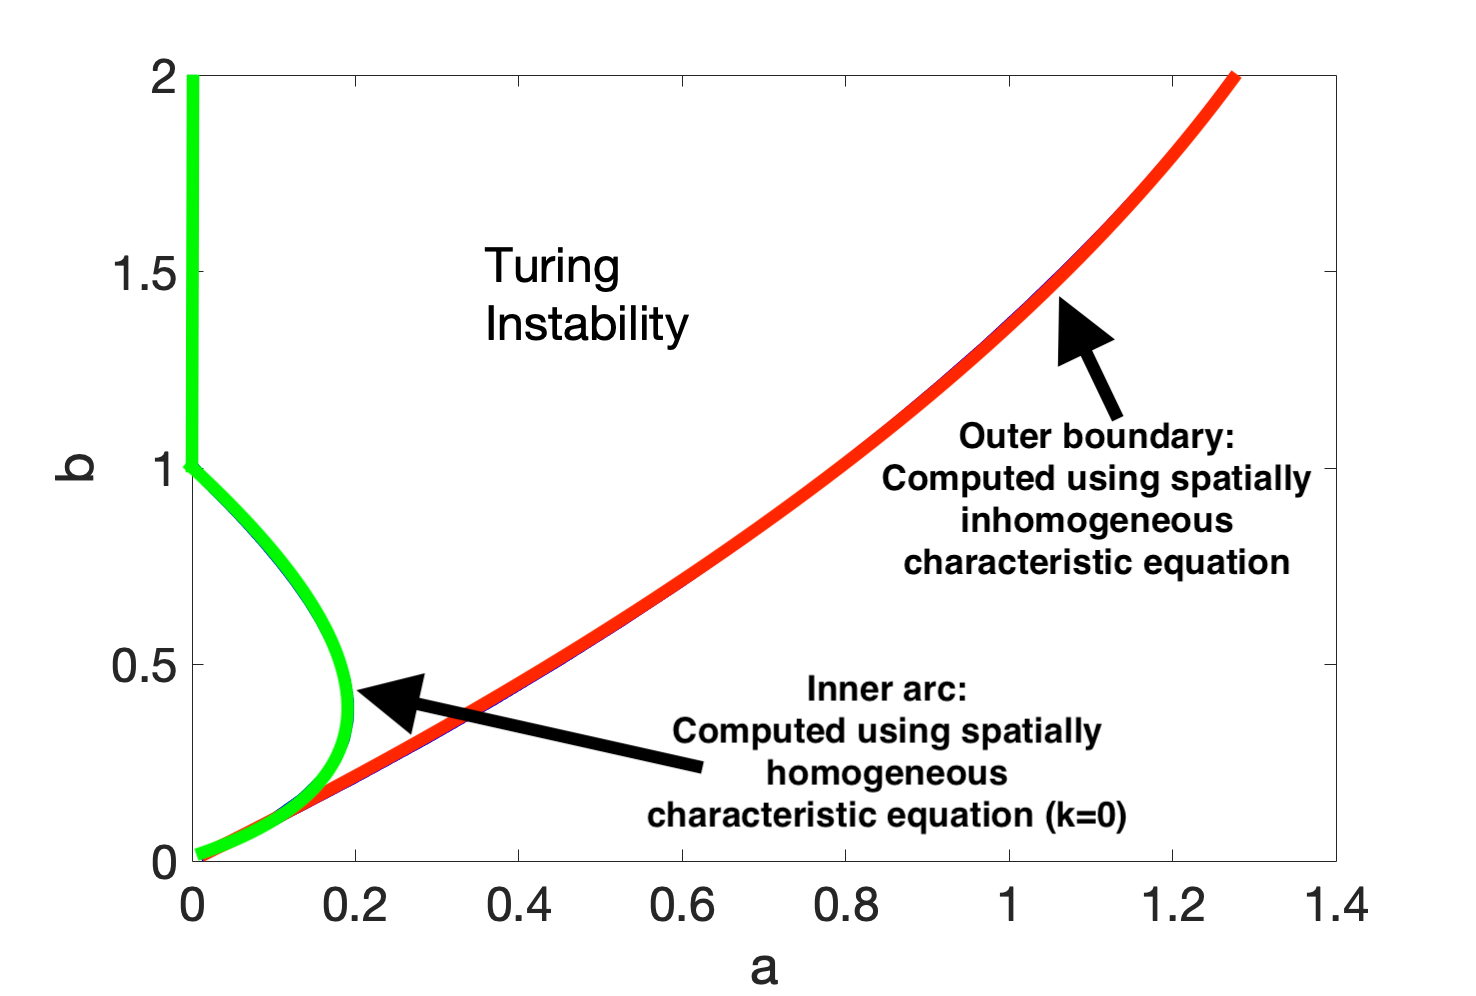
\includegraphics[width=7cm,height = 5.5cm]{bif0.png}
        \caption{Stability lines for $\tau=0$ computed by solving characteristic equation \eqref{characfix} with $\epsilon^2=0.001$, $L=30\sqrt{0.05}$.}
        \label{fig:bif0}
    \end{subfigure}
    \hfill
    \begin{subfigure}[b]{0.47\textwidth}
        \centering
        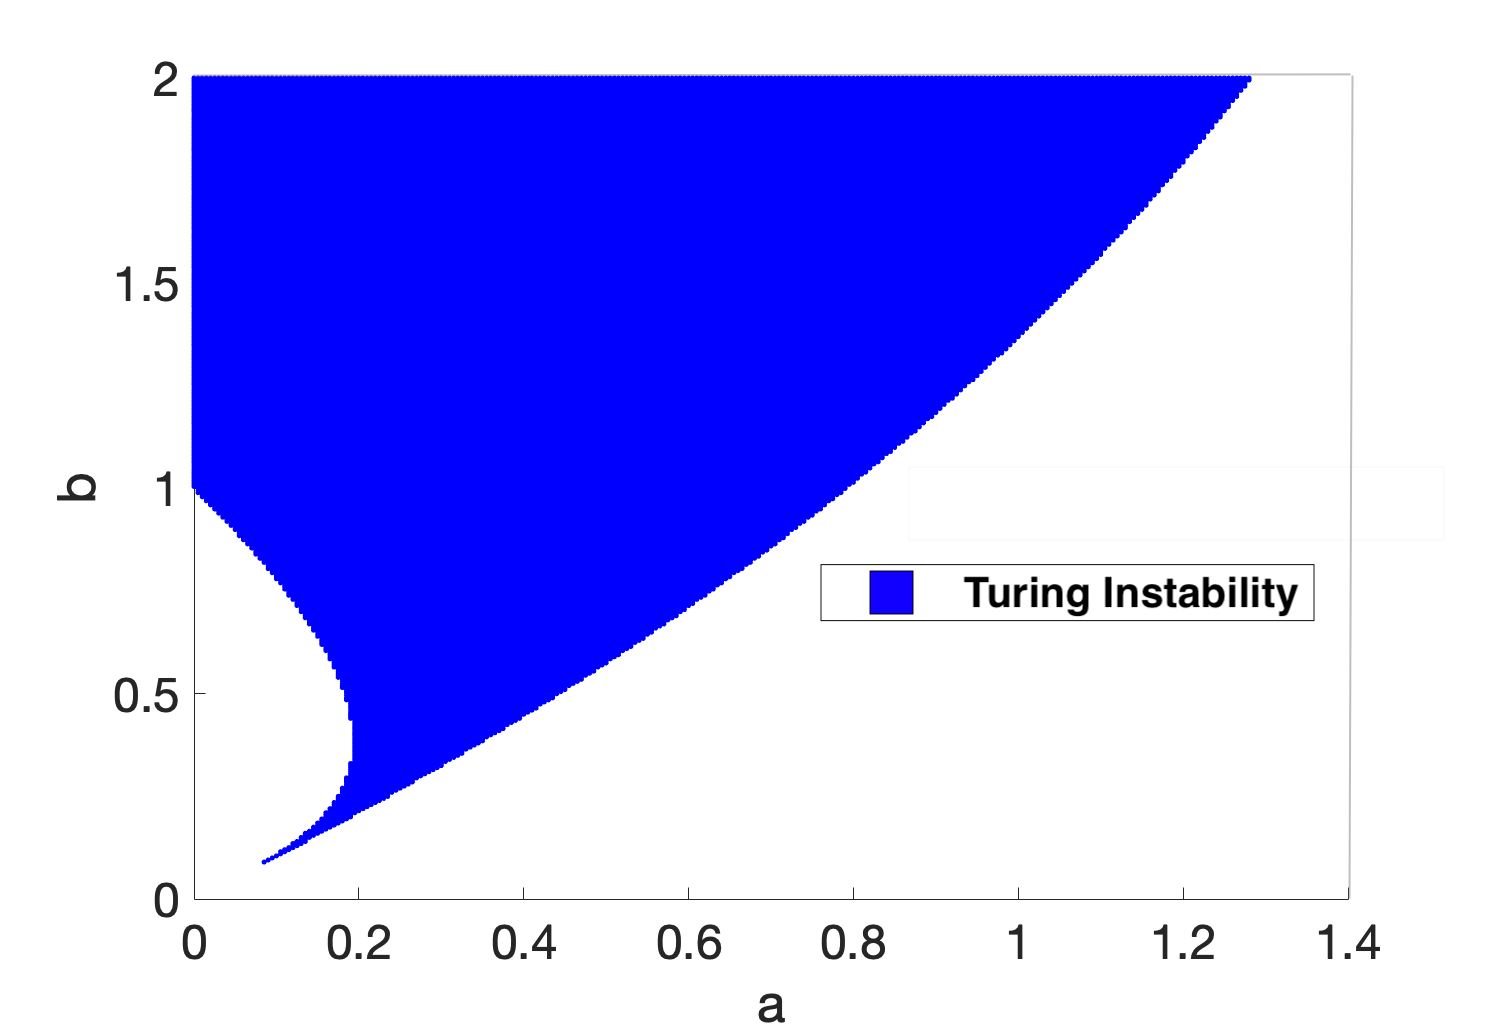
\includegraphics[width=7cm,height = 5.5cm]{turingspace.png}
        \caption{Turing space as in figure \ref{fig:turingspace} plotted from parameters $(a,b)$ satisfying conditions \eqref{cond1} and \eqref{cond2}.}
        \label{}
    \end{subfigure}
    \caption{Comparison of Turing instability region for $\tau=0$ computed via characterstic equation against Turing instability region computed via conditions \eqref{cond1} and \eqref{cond2}.}
    \label{fig:tspace1}
\end{figure}

Figure \ref{fig:tspacetau} shows the stability curves computed for a varying $\tau\in\{0,0.5,1,1.5\}$. It can be seen that, whilst the outer boundary computed from the characteristic equation for the spatially inhomogeneous model stays the same, the inner arc computed from using the characteristic equation from the spatially homogeneous model shifts to the left, increasing the region of parameter space for which Turing instabilities can occur. This observation matches the results produced in \cite{william} for the spatially homogeneous LI model. This is also a similar result to that observed in \cite{fadai} for the Gierer-Meinhardt model. We see that for the LI model where delay-terms are placed solely in the activator dynamics, time delay acts as a stabilising agent for pattern formation and increases the parameter space where pattern formation will occur.
\begin{figure}[H]
        \centering
        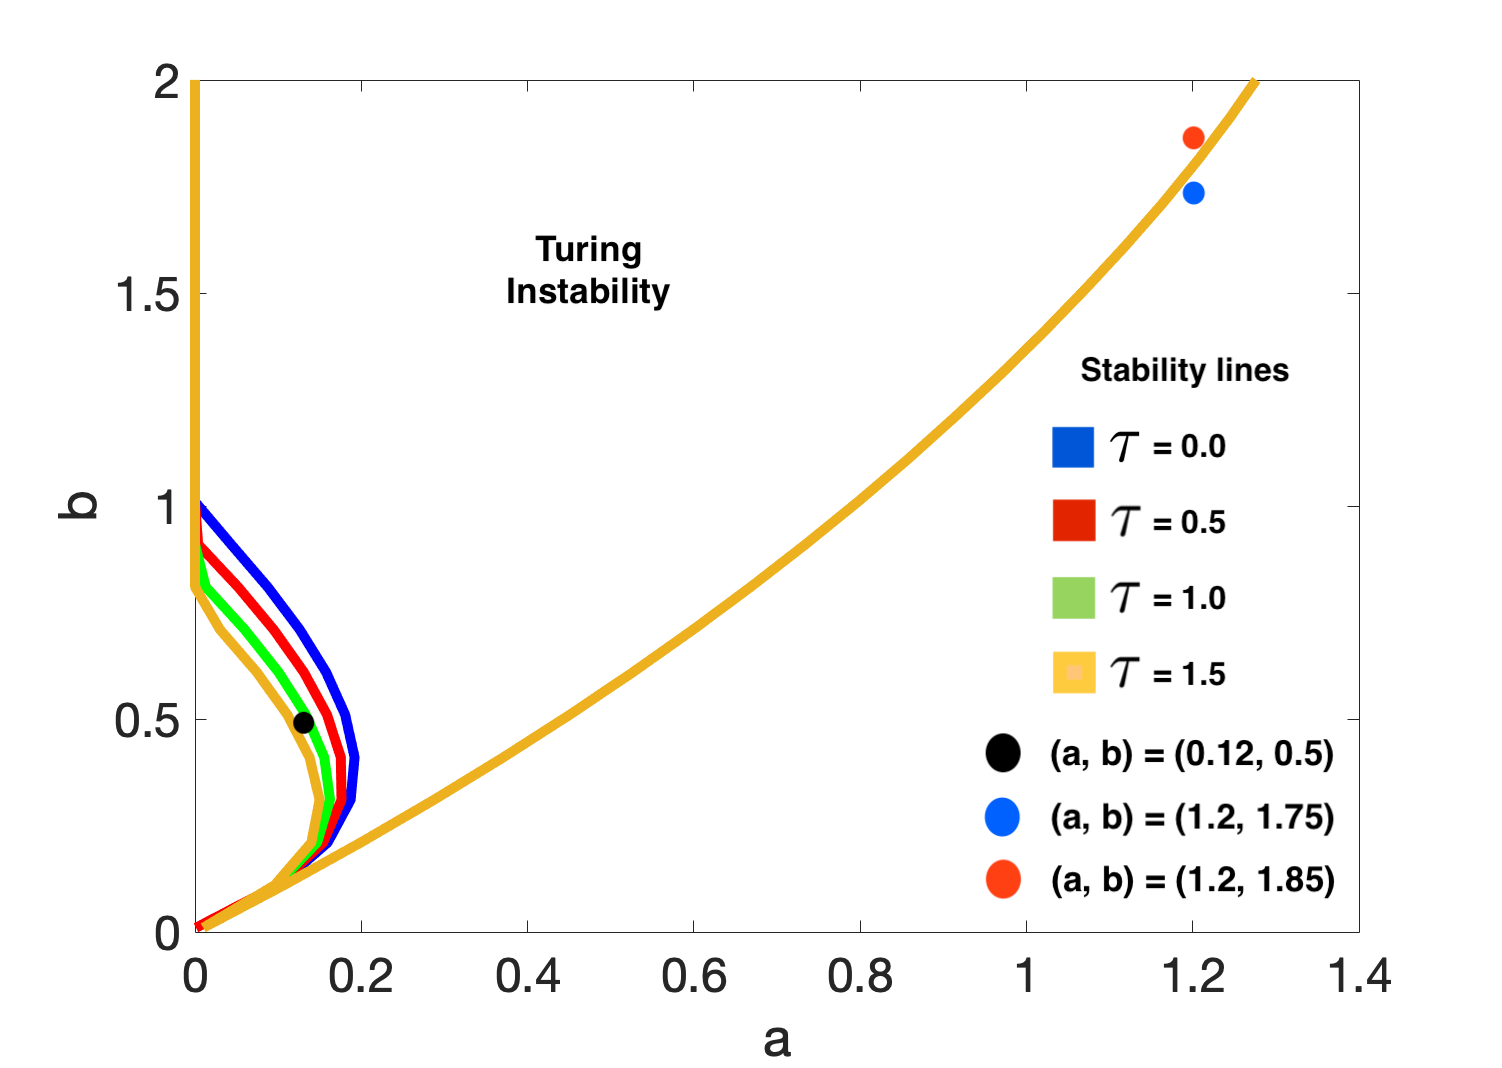
\includegraphics[width=12cm,height = 9cm]{tspacetau.png}
        \caption{Stability lines for $\tau\in\{0,0.5,1,1.5\}$ computed using characteristic equation. $\epsilon^2=0.001$, $L=30\sqrt{0.05}$.}
        \label{fig:tspacetau}
\end{figure}
We verify the results in figure \ref{fig:tspacetau} through numerical simulations. Three parameter points, $(a,b)=\{(0.12,0.5),(1.2,1.75),(1.2,1.85)\}$ are indicated in figure \ref{fig:tspacetau}. At $(a,b,\tau)=(0.12,0.5,0)$, linear theory suggests that there will be no pattern formation, but at $(a,b,\tau)=(0.12,0.5,1.5)$ there will be a Turing instability and thus patterns will form.
The parameter region in the bottom left of the parameter space is a delicate region that can exhibit both Turing and Hopf bifurcations, leading to complex spatio-temporal behaviours. This type of dynamics in reaction-diffusion systems has been studied more extensively in \cite{krausefixed,jiang}. Although the linear theory is unable to provide information about these intricate nonlinear dynamics, it can predict the expected type of behaviour for certain parameter values. To show a change in behaviour as $\tau$ changes, from a temporally oscillating solution, to one exhibiting a Turing pattern, we increase the diffusive ratio to $\epsilon^2=0.1$. This result can be seen in figure \ref{fig:testturing}. The linear theory also suggests that for all $\tau\in\{0,0.5,1,1.5\}$, pattern formation will occur for $(a,b)=(1.2,1.85)$, but not for $(a,b)=(1.2,1.75)$. Figures \ref{fig:testturing2} and \ref{fig:testturing3} show the results for numerical simulations at $(a,b)=\{(1.2,1.75),(1.2,1.85)\}$ for $\tau=\{0,0.5,1,1.5\}$.
\begin{figure}[h]
    \centering
    \begin{subfigure}[b]{0.45\textwidth}
        \centering
        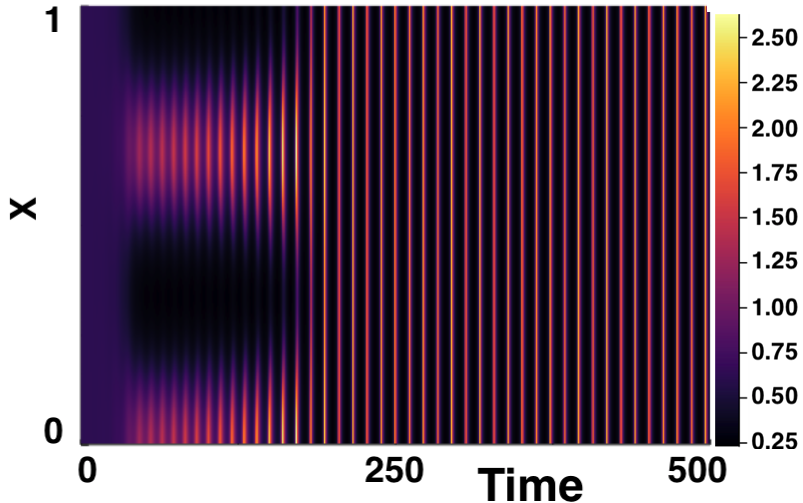
\includegraphics[width=7cm,height=5cm]{toscill.png}
        \caption{$\tau=0$. Oscillations seen.}
        \label{}
    \end{subfigure}
    \hfill
    \begin{subfigure}[b]{0.45\textwidth}
        \centering
        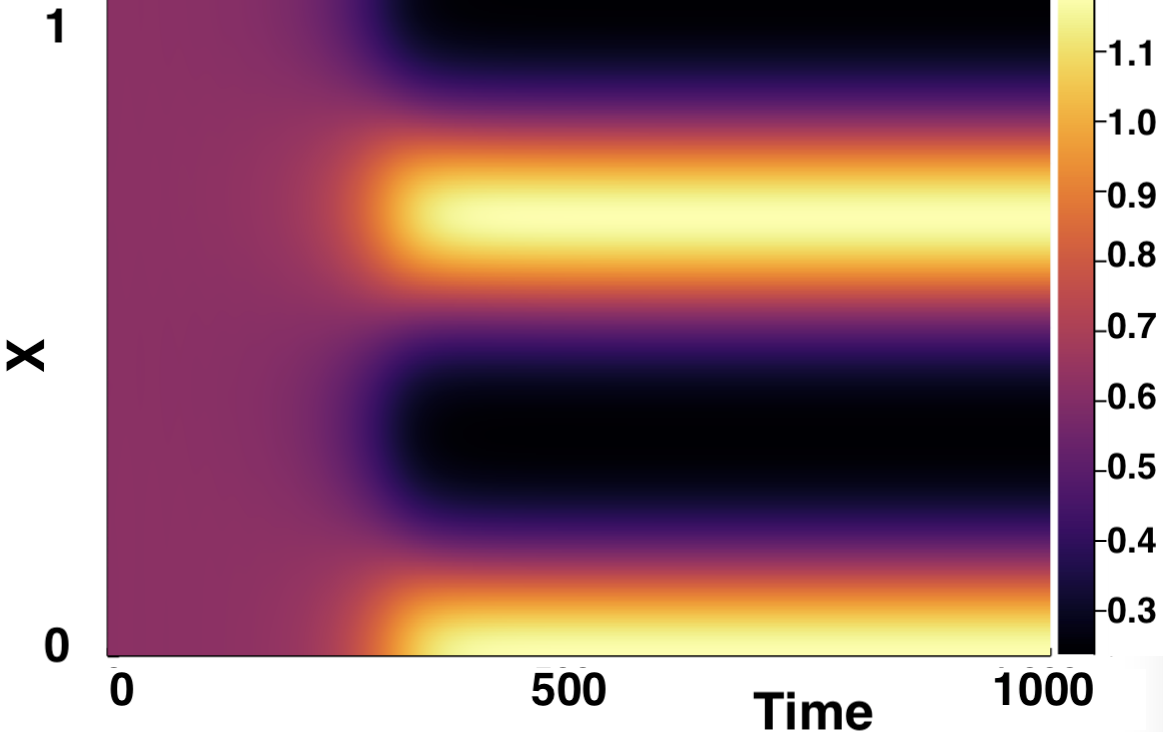
\includegraphics[width=7cm,height=5cm]{tpattpred.png}
        \caption{$\tau=1.5$. Pattern formation seen.}
        \label{}
    \end{subfigure}
    \caption{Numerical simulations produced with parameters $(a,b)=(0.12,0.5)$, for $\tau=0,1.5$. $\epsilon^2=0.1$ and $L=30\sqrt{0.05}$. Linear theory in figure \ref{fig:tspacetau} suggests we see pattern formation at $\tau=1.5$ but not at $\tau=0$.}
    \label{fig:testturing}
\end{figure}

\begin{figure}[H]
    \centering
    \begin{subfigure}[b]{0.45\textwidth}
        \centering
        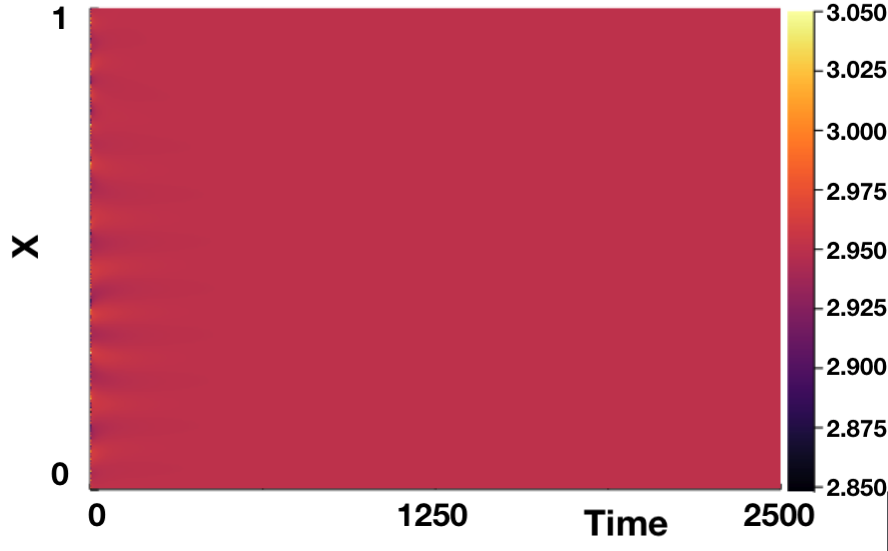
\includegraphics[width=7cm,height=4cm]{p3t0.png}
        \caption{$\tau=0$.}
        \label{}
    \end{subfigure}
    \hfill
    \begin{subfigure}[b]{0.45\textwidth}
        \centering
        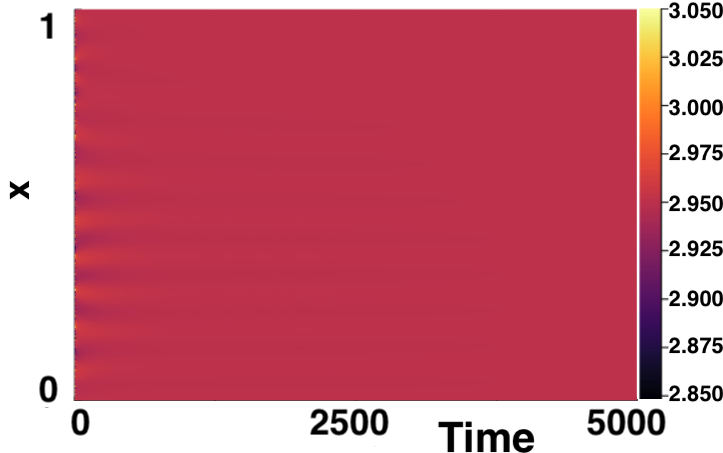
\includegraphics[width=7cm,height=4cm]{p3t05.png}
        \caption{$\tau=0.5$}
        \label{}
    \end{subfigure}
    \hfill
    \begin{subfigure}[b]{0.45\textwidth}
        \centering
        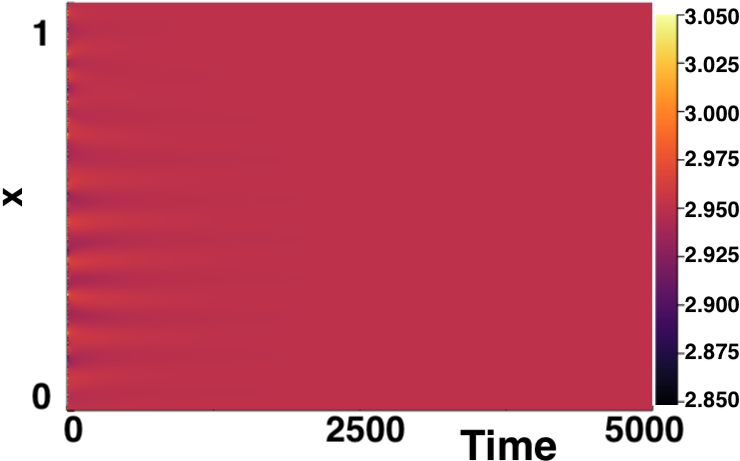
\includegraphics[width=7cm,height=4cm]{p3t1.png}
        \caption{$\tau=1$}
        \label{}
    \end{subfigure}
    \hfill
    \begin{subfigure}[b]{0.45\textwidth}
        \centering
        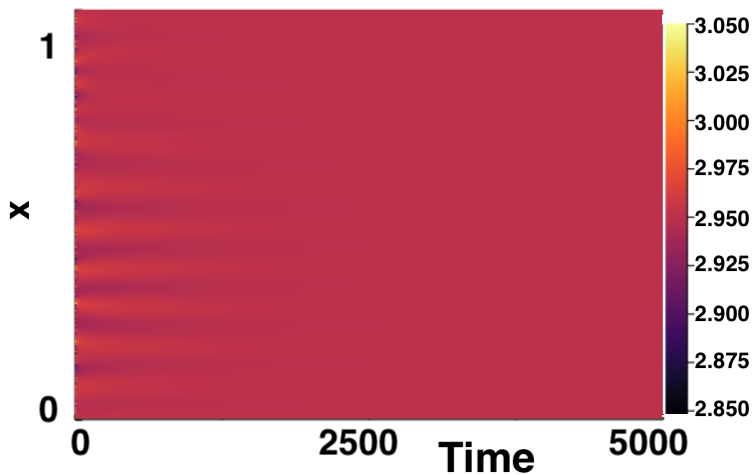
\includegraphics[width=7cm,height=4cm]{p3t15.png}
        \caption{$\tau=1.5$.}
        \label{}
    \end{subfigure}
    \caption{Numerical simulations for $(a,b)=(1.2,1.75)$. $\epsilon^2=0.001$ and $L=30\sqrt{0.05}$.  We see no pattern formation for $\tau\in\{0,0.5,1,1.5\}$ as suggested by linear theory, seen in figure \ref{fig:tspacetau}.}
    \label{fig:testturing2}
\end{figure}

\begin{figure}[H]
    \centering
    \begin{subfigure}[b]{0.45\textwidth}
        \centering
        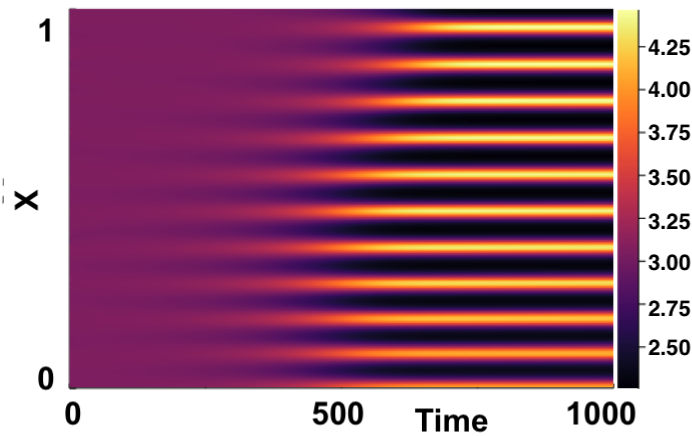
\includegraphics[width=7cm,height=4cm]{p2t0.png}
        \caption{$\tau=0$.}
        \label{}
    \end{subfigure}
    \hfill
    \begin{subfigure}[b]{0.45\textwidth}
        \centering
        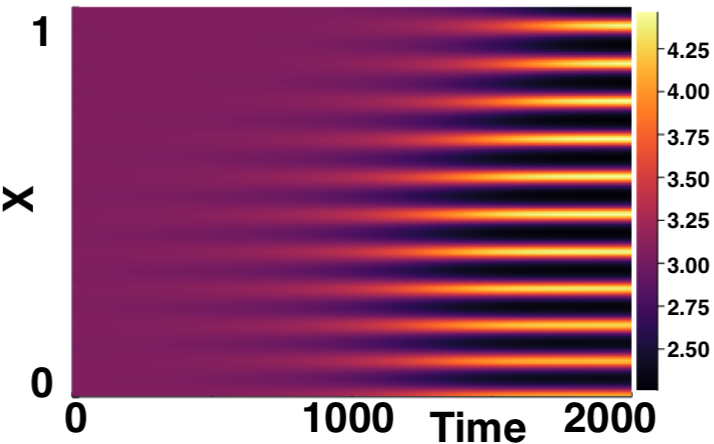
\includegraphics[width=7cm,height=4cm]{p2t05.png}
        \caption{$\tau=0.5$}
        \label{}
    \end{subfigure}
    \hfill
    \begin{subfigure}[b]{0.45\textwidth}
        \centering
        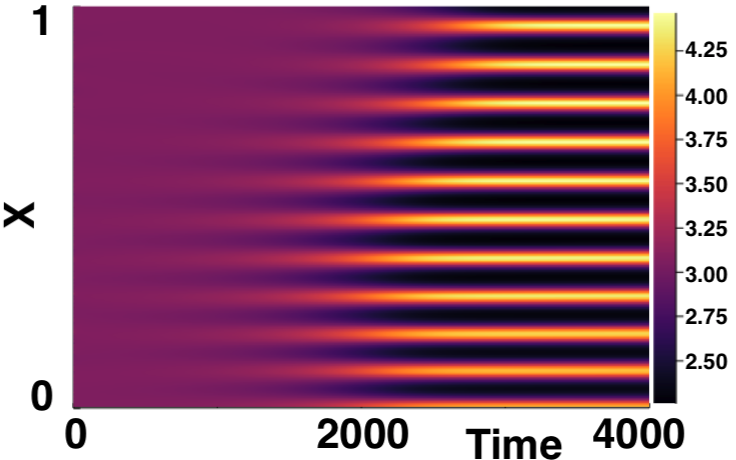
\includegraphics[width=7cm,height=4cm]{p2t1.png}
        \caption{$\tau=1$}
        \label{}
    \end{subfigure}
    \hfill
    \begin{subfigure}[b]{0.45\textwidth}
        \centering
        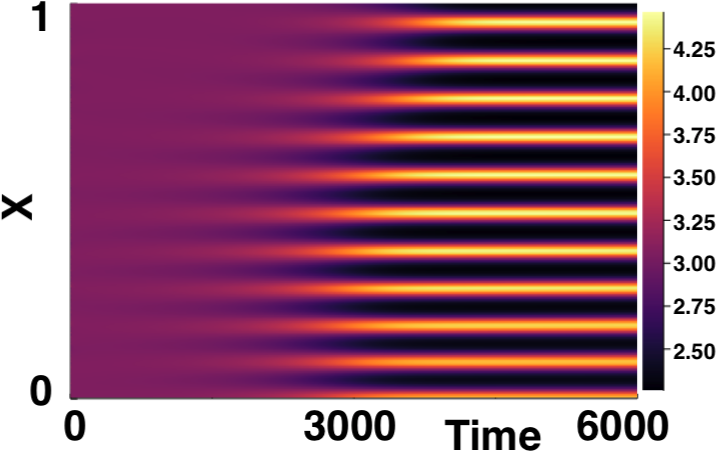
\includegraphics[width=7cm,height=4cm]{p2t15.png}
        \caption{$\tau=1.5$.}
        \label{}
    \end{subfigure}
    \caption{Numerical simulations for $(a,b)=(1.2,1.85)$. $\epsilon^2=0.001$ and $L=30\sqrt{0.05}$. We see pattern formation on an increasing time-scale for $\tau\in\{0,0.5,1,1.5\}$ as suggested by linear theory, seen in figure \ref{fig:tspacetau}. Increasing time-scale seen from changing $x$-axis limits.}
    \label{fig:testturing3}
\end{figure}

Figure \ref{fig:tspacetau} shows how the time delay affects the region of Turing instability, but it provides no information as to how $\max_k(\Re(\lambda_k))$ varies as $\tau$ increases over the $(a,b)$ parameter space. In figure \ref{fig:lambdavary} we plot a heatmap of $\max_k(\Re(\lambda_k))$ over the $(a,b)$ parameter space for varying $\tau\in\{0,0.5,1,1.5\}$. Overlayed onto these plots are contour lines corresponding to where $\Re(\lambda_0)=0$ and $\max_k(\Re(\lambda_k))=0$, highlighting the Turing instability region. The $\max_k$ taken over $k\in[0,50]$ at regular discrete intervals of $1$.
\begin{figure}[H]
    \centering
    \begin{subfigure}[b]{0.45\textwidth}
        \centering
        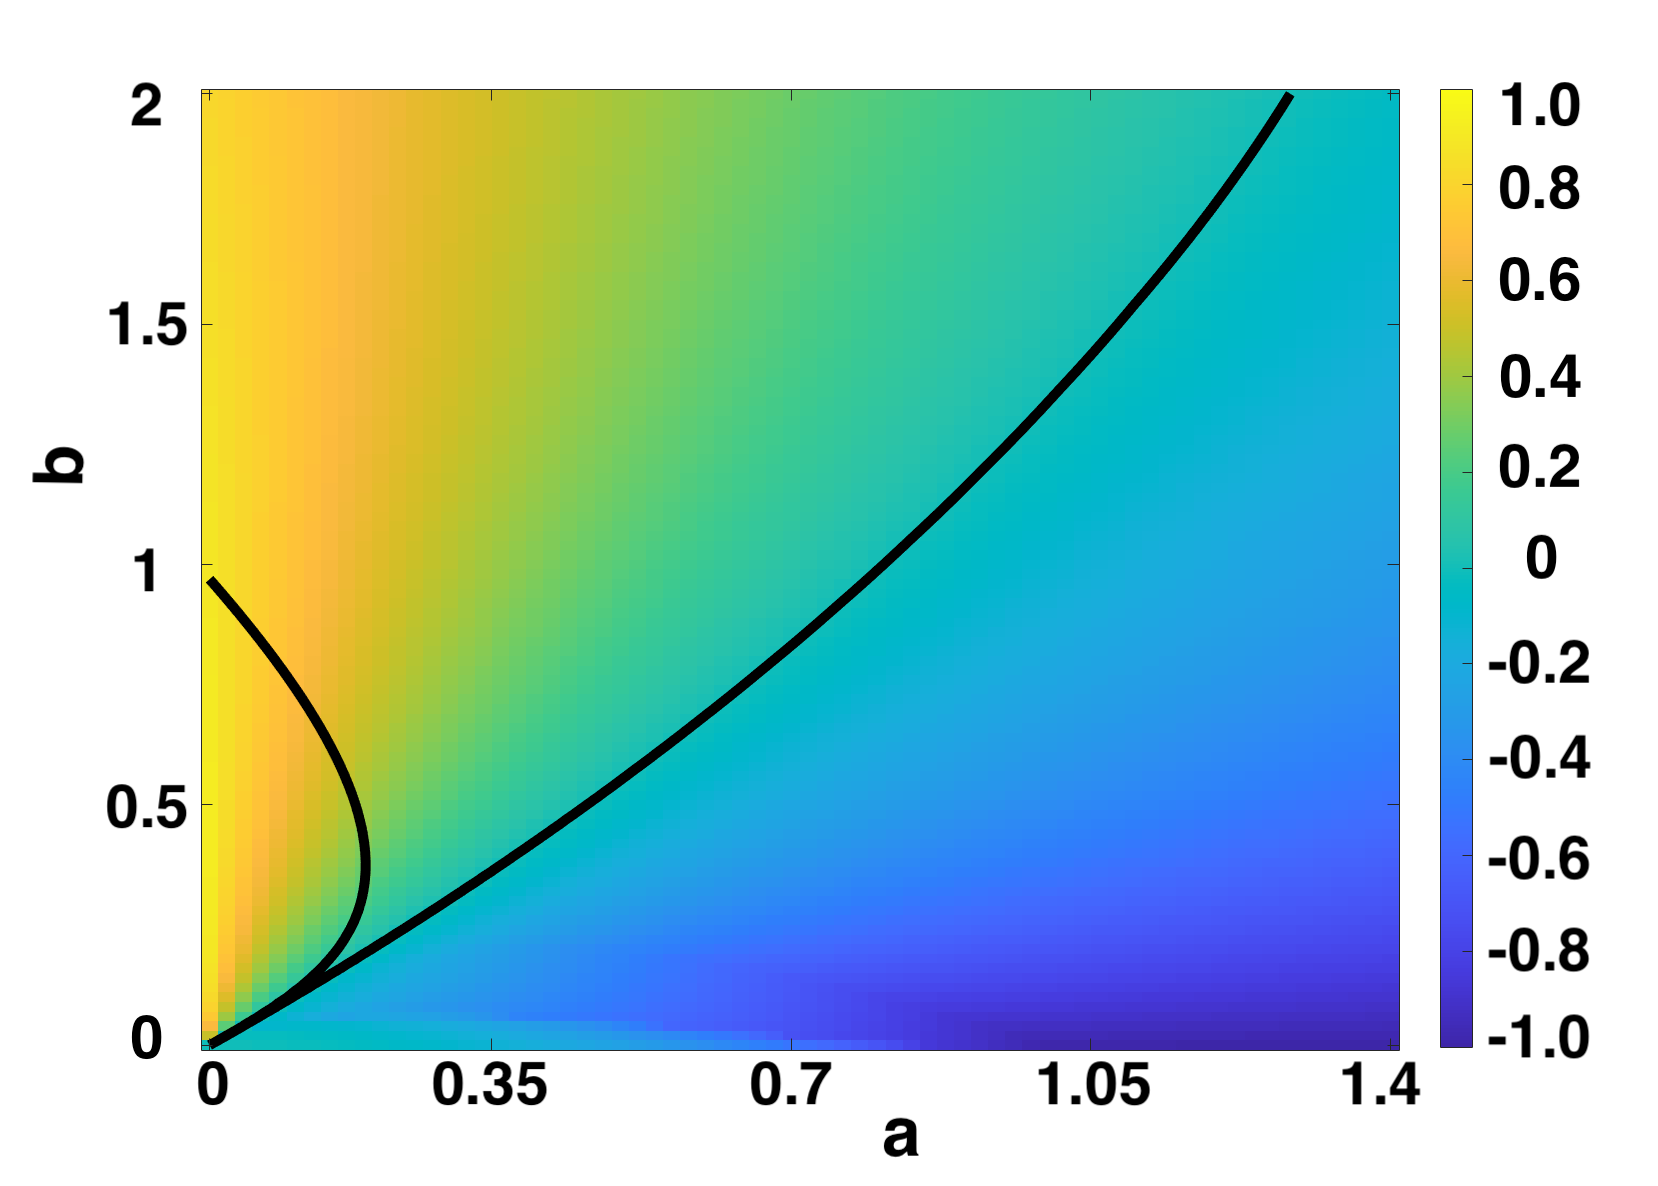
\includegraphics[width=7cm,height=5cm]{tau0bif.png}
        \caption{$\tau=0$.}
        \label{}
    \end{subfigure}
    \hfill
    \begin{subfigure}[b]{0.45\textwidth}
        \centering
        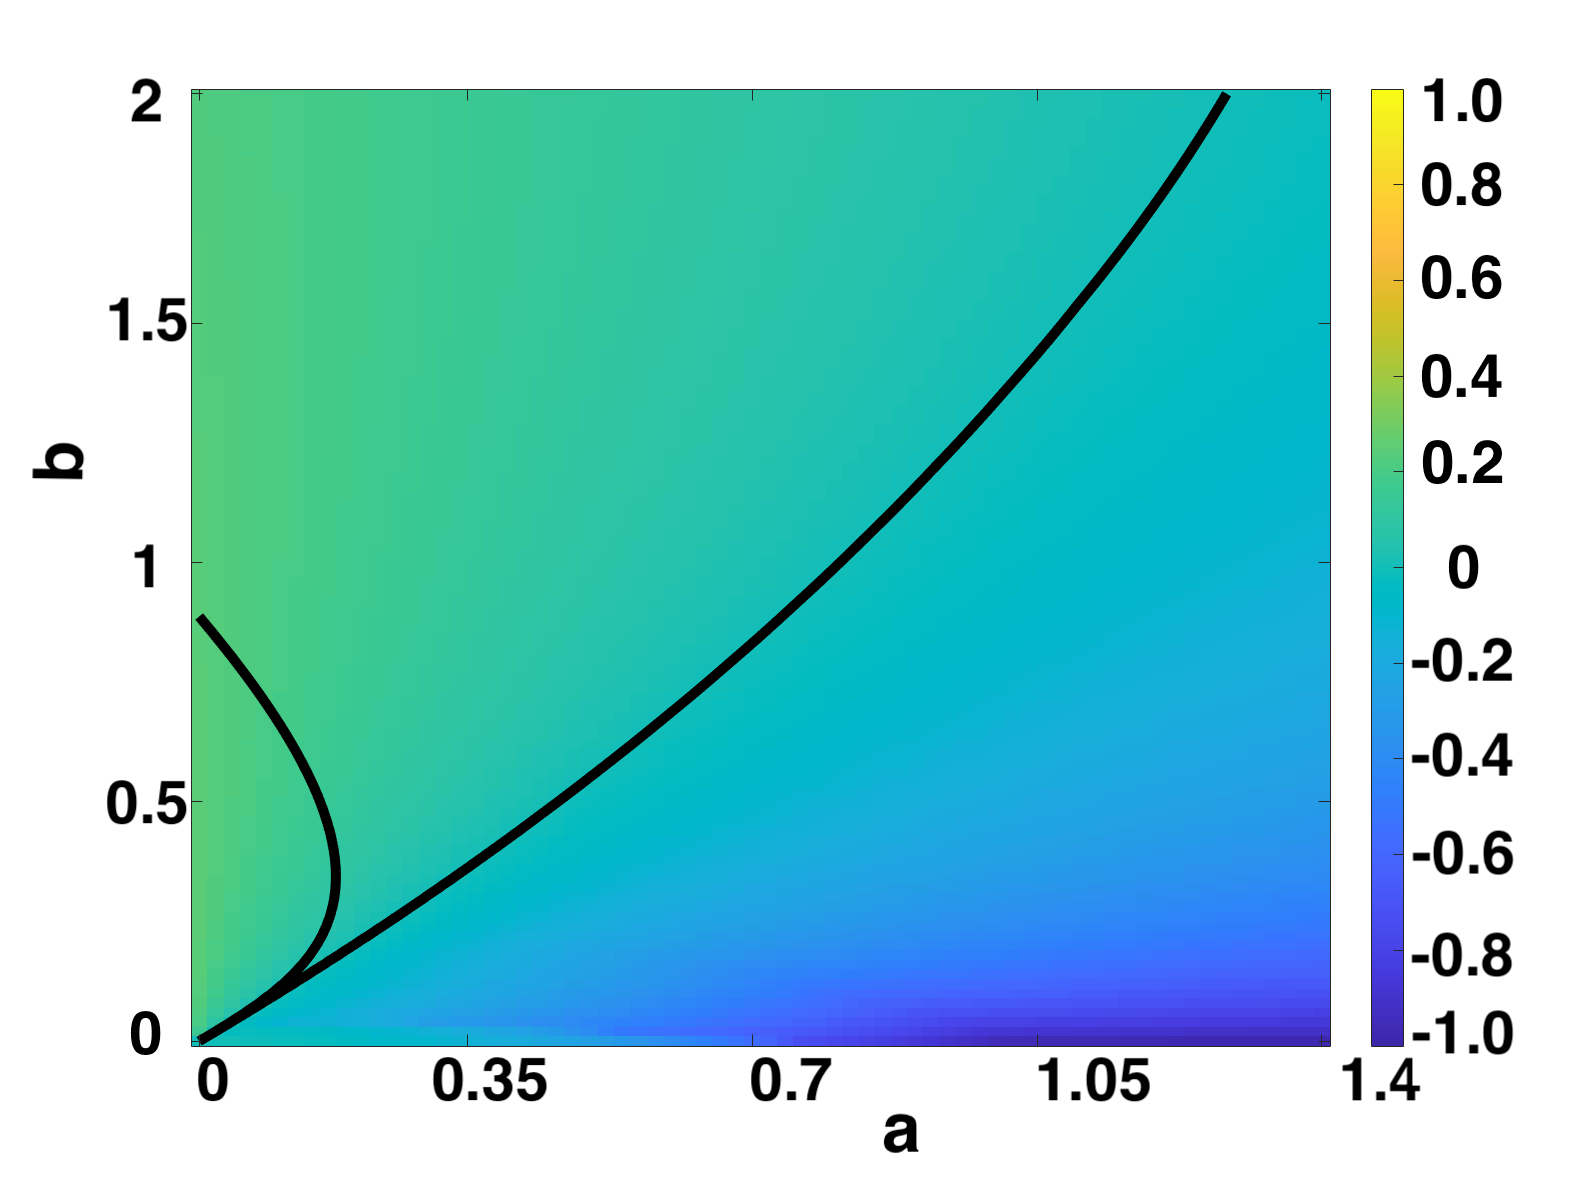
\includegraphics[width=7cm,height=5cm]{tau05bif.png}
        \caption{$\tau=0.5$}
        \label{}
    \end{subfigure}
    \hfill
    \begin{subfigure}[b]{0.45\textwidth}
        \centering
        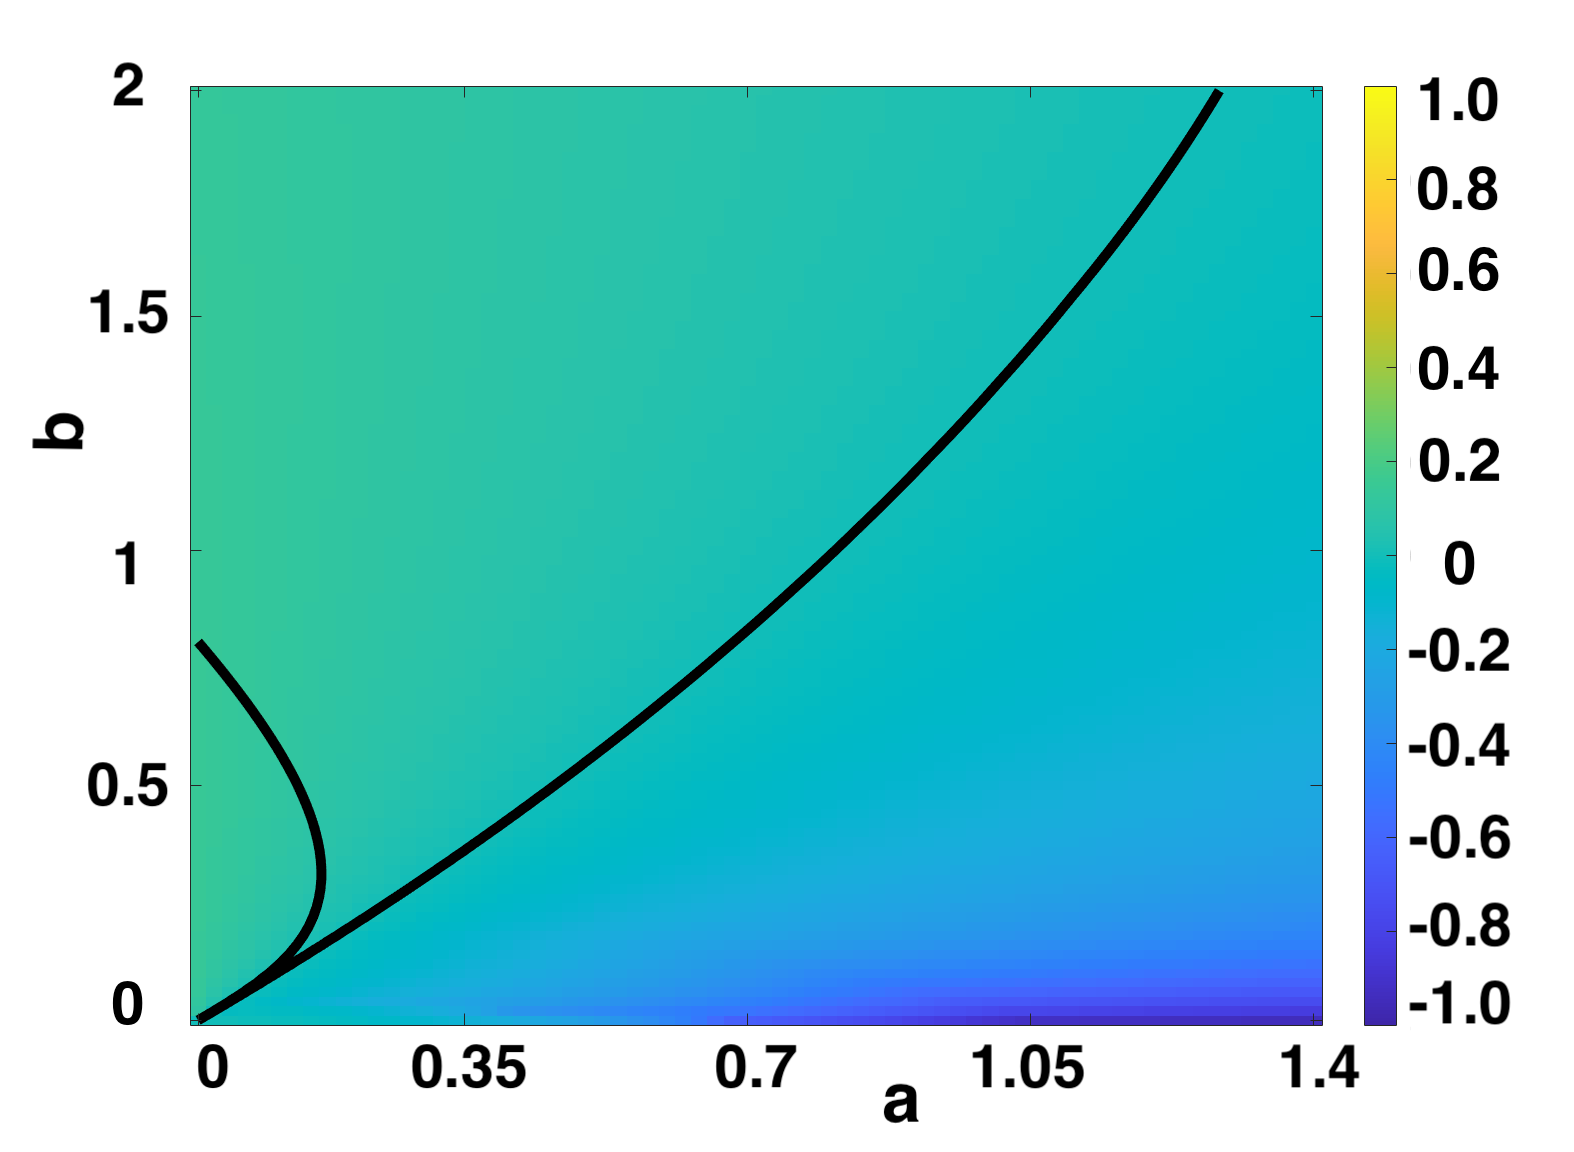
\includegraphics[width=7cm,height=5cm]{tau1bif.png}
        \caption{$\tau=1$}
        \label{}
    \end{subfigure}
    \hfill
    \begin{subfigure}[b]{0.45\textwidth}
        \centering
        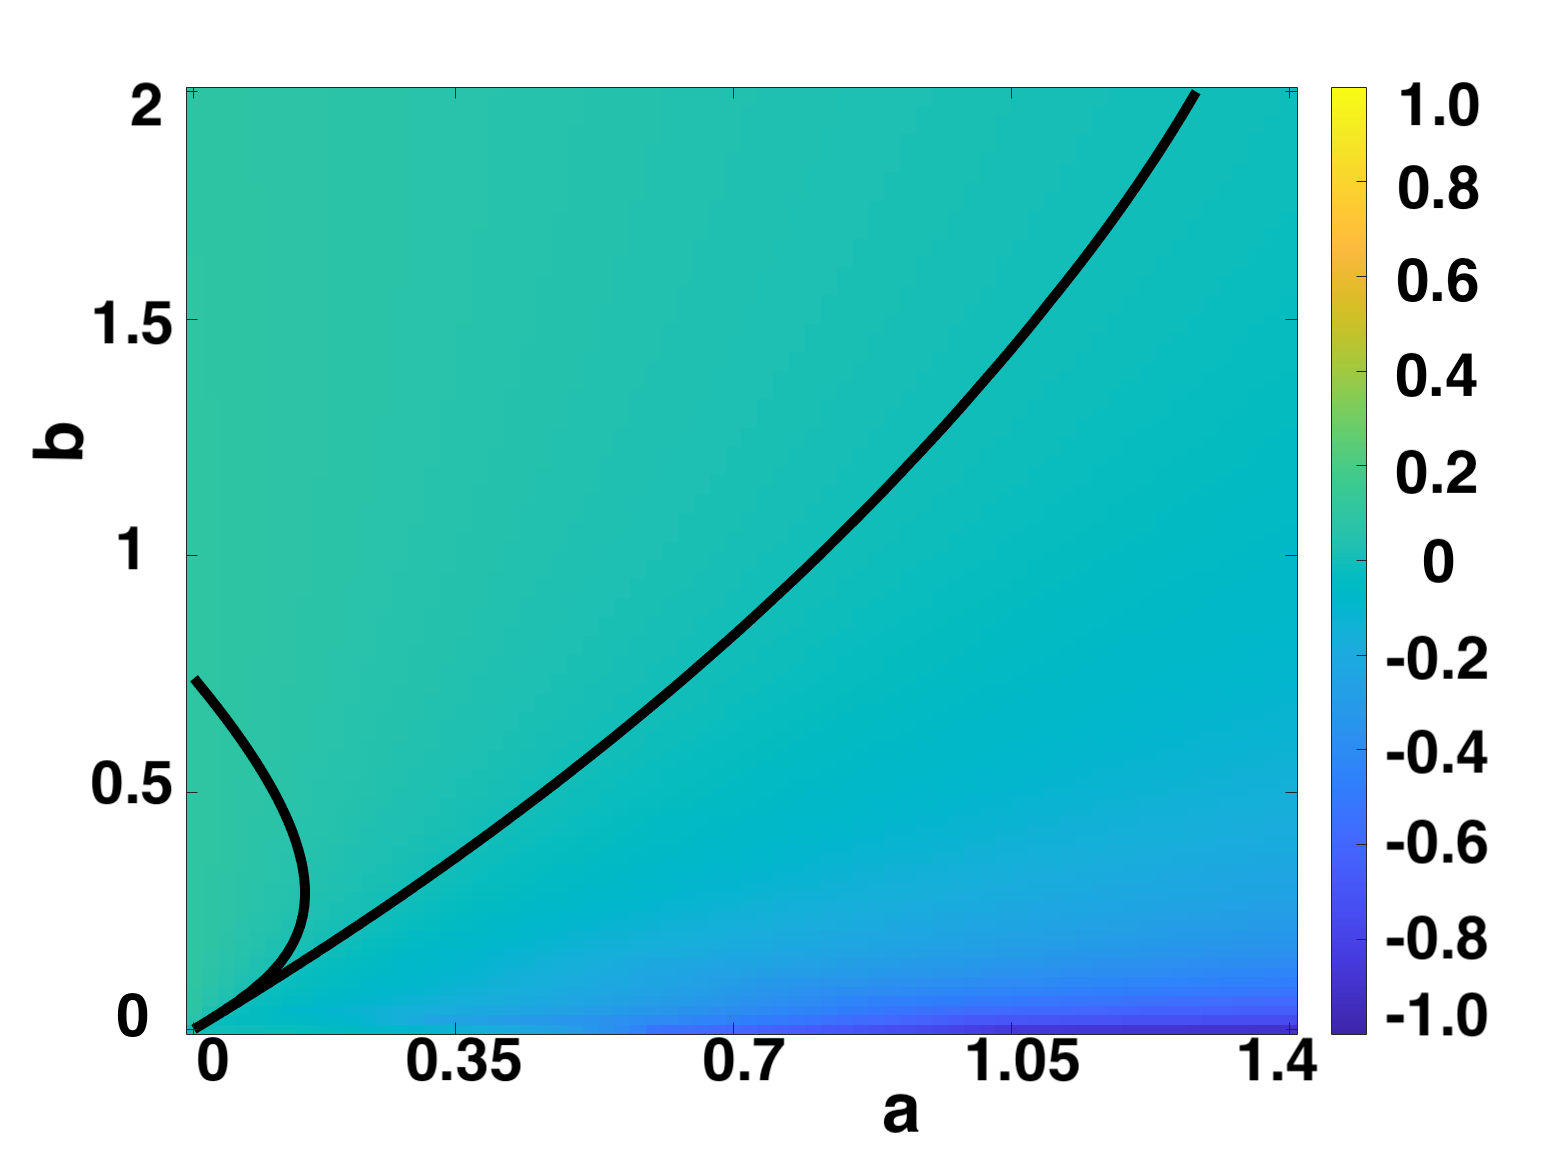
\includegraphics[width=7cm,height=5cm]{tau15bif.png}
        \caption{$\tau=1.5$.}
        \label{}
    \end{subfigure}
    \caption{$\max_k(\Re(\lambda_k))$ computed over $(a,b)$ parameter space by solving characteristic equation \eqref{characfix}, with $\epsilon^2=0.001$, $L=30\sqrt{0.05}$. As $\tau$ increases, $|\max_k(\Re(\lambda_k))|$ decreases. Contour lines for $\Re(\lambda_0)=0$ and $\max_k(\Re(\lambda))=0$ overlayed, indicated Turing instability region.}
    \label{fig:lambdavary}
\end{figure}
As $\tau$ increases, it can be seen that the absolute value $|\max_k(\Re((\lambda_k)))|$ also decreases. This suggests that for $(a,b)$ values within the Turing instability region, pattern formation will take longer to occur. It also suggests however that for $(a,b)$ such that $\max_k(\Re(\lambda_k))<0$, it will take a longer time for the eigenfunctions with modes $k\neq0$ to decay to a spatially homogeneous steady-state. We see this behaviour in figure \ref{fig:testturing2}, where it can be seen that the time taken for the initial perturbation to fully decay back to a spatially homogeneous steady-state increases as $\tau$ increases. Figure \ref{fig:fixbif2} shows analogous bifurcation diagrams as in figure \ref{fig:lambdavary}, but with $\epsilon^2=0.1$. We note that as the ratio, $\epsilon^2$, of diffusion constants in the reaction-diffusion constant moves closer to $1$, the region of parameter space exhibiting Turing instability decreases. It can be observed however that altering $\epsilon^2$ does not change the effect that an increasing $\tau$ has on $\max_k(\Re(\lambda_k))$, and that increasing the delay $\tau$ continues to act as a stabilising agent for Turing instabilities, with a shifting of the spatially homogeneous inner arc.

\begin{figure}[H]
    \centering
    \begin{subfigure}[b]{0.45\textwidth}
        \centering
        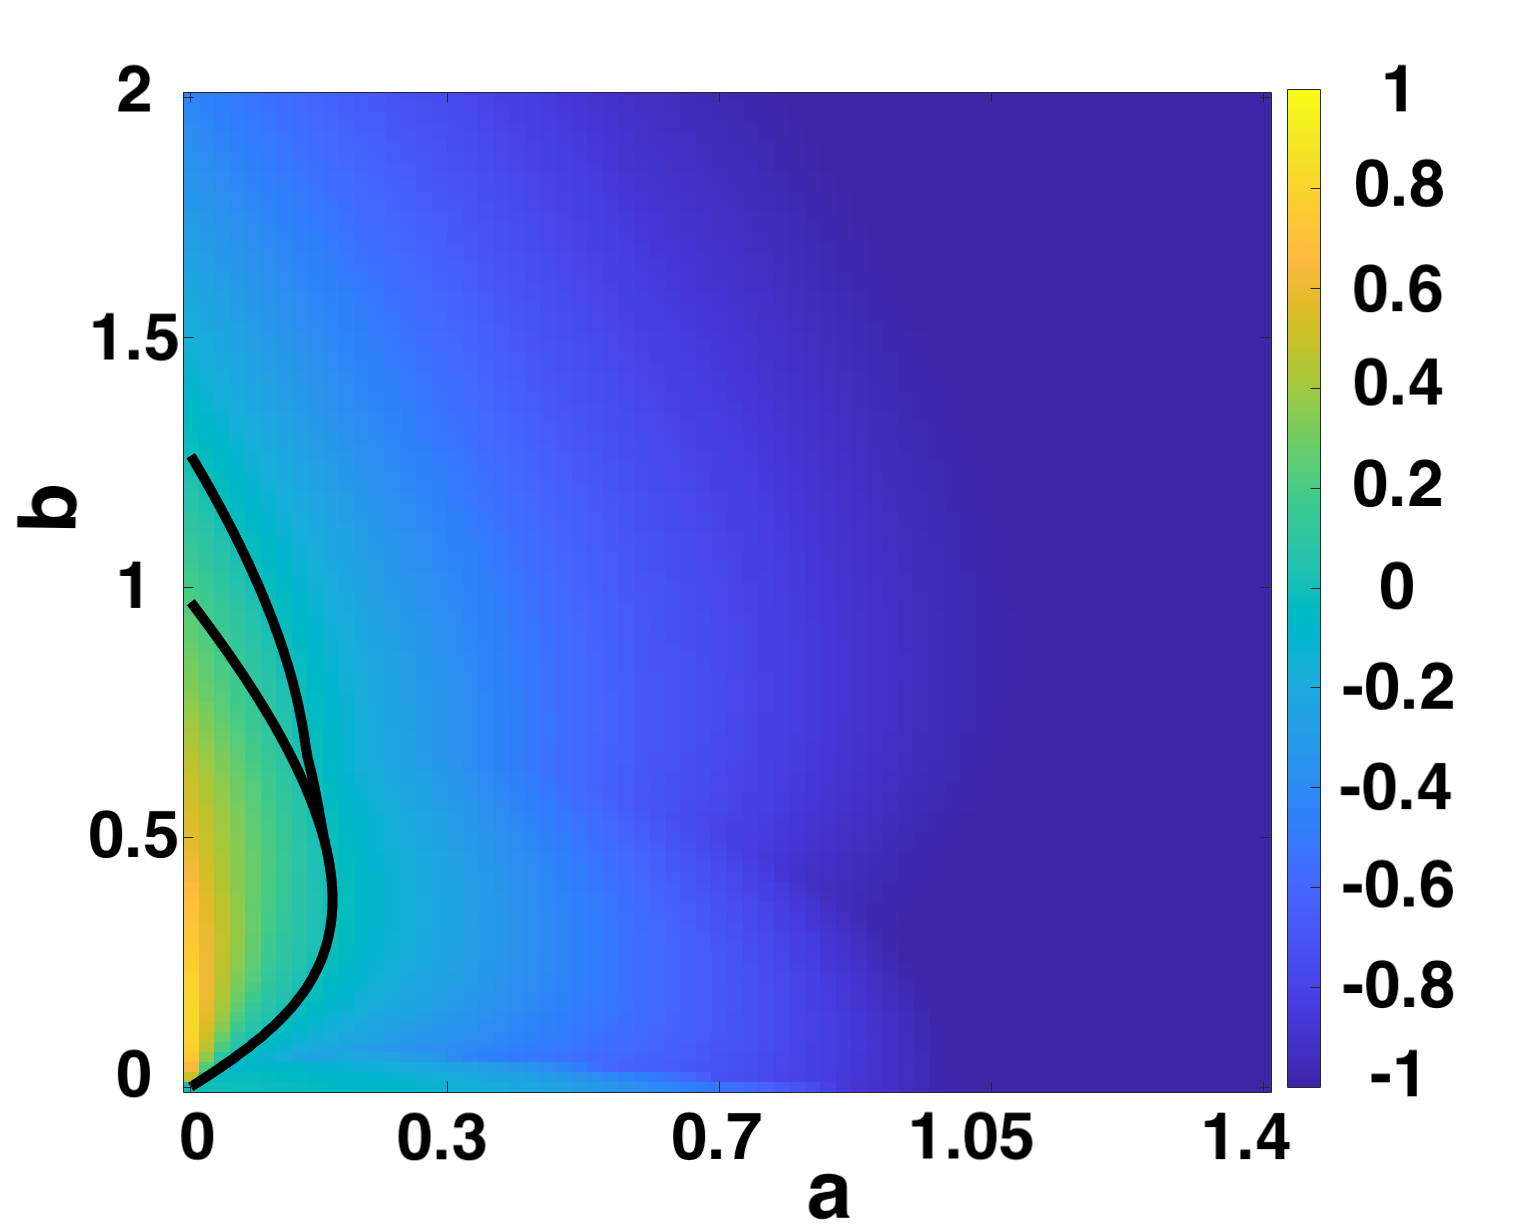
\includegraphics[width=7cm,height=5cm]{fixbif21.png}
        \caption{$\tau=0$.}
        \label{}
    \end{subfigure}
    \hfill
    \begin{subfigure}[b]{0.45\textwidth}
        \centering
        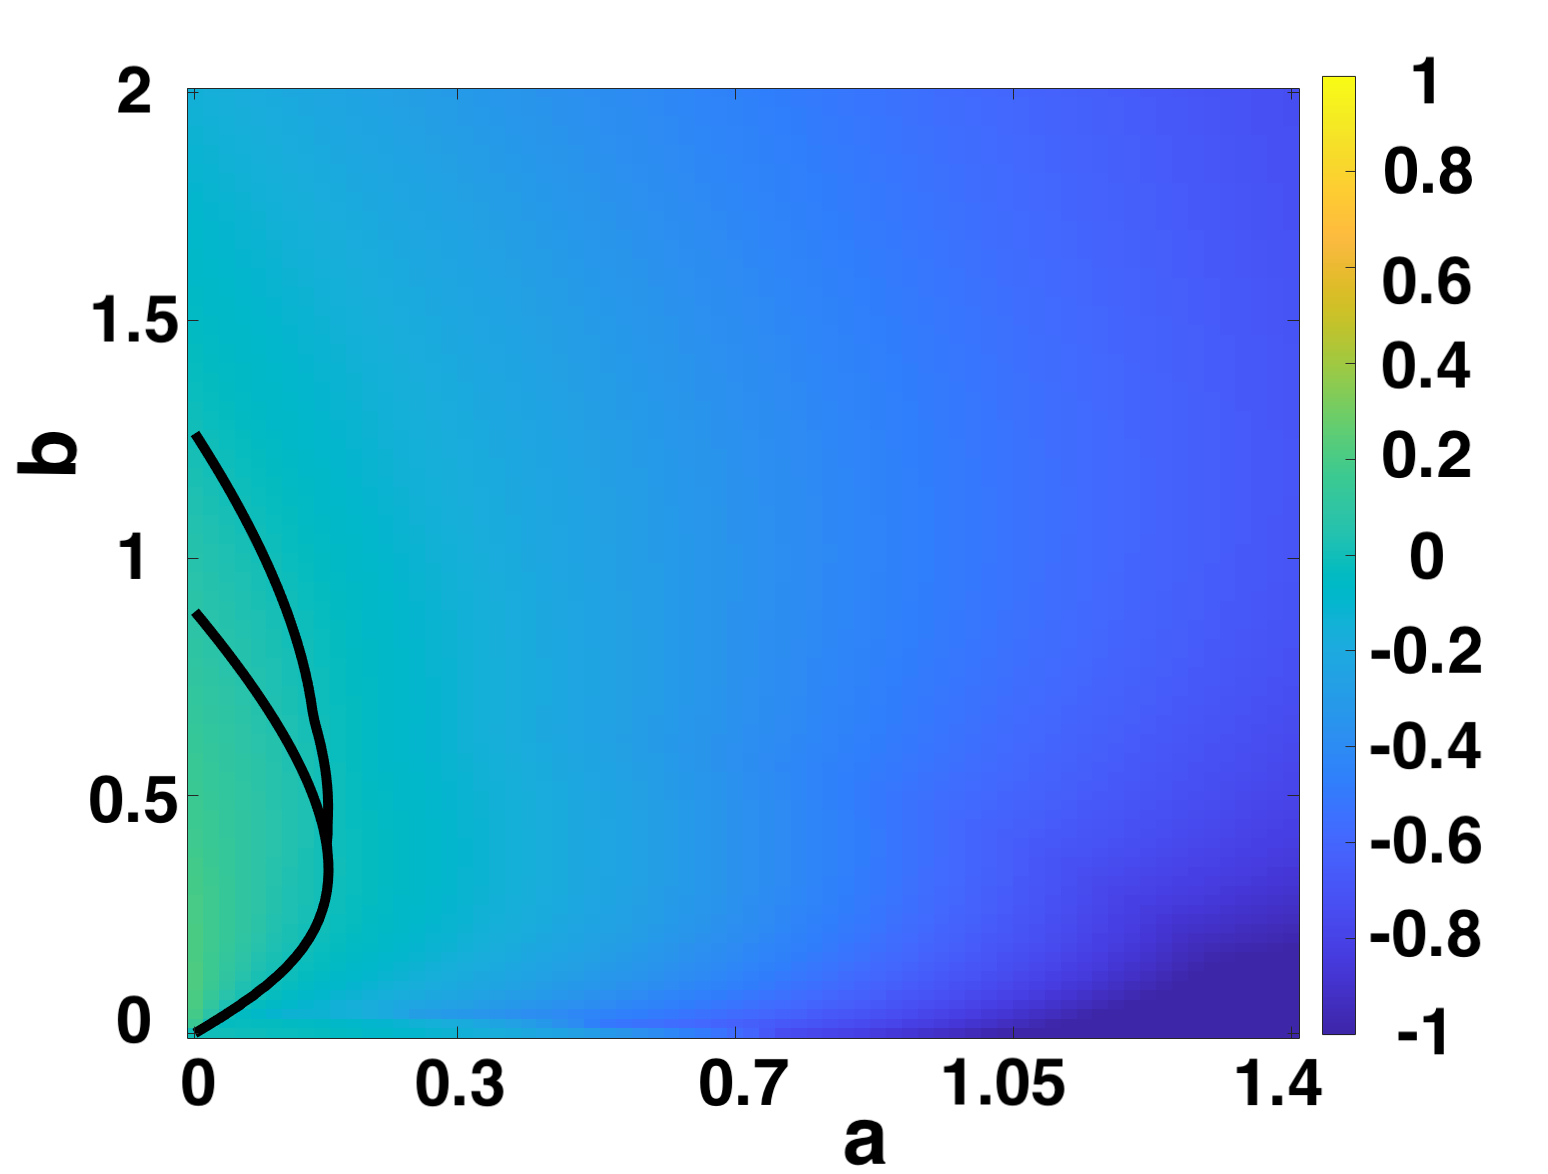
\includegraphics[width=7cm,height=5cm]{fixbif22.png}
        \caption{$\tau=0.5$}
        \label{}
    \end{subfigure}
    \hfill
    \begin{subfigure}[b]{0.45\textwidth}
        \centering
        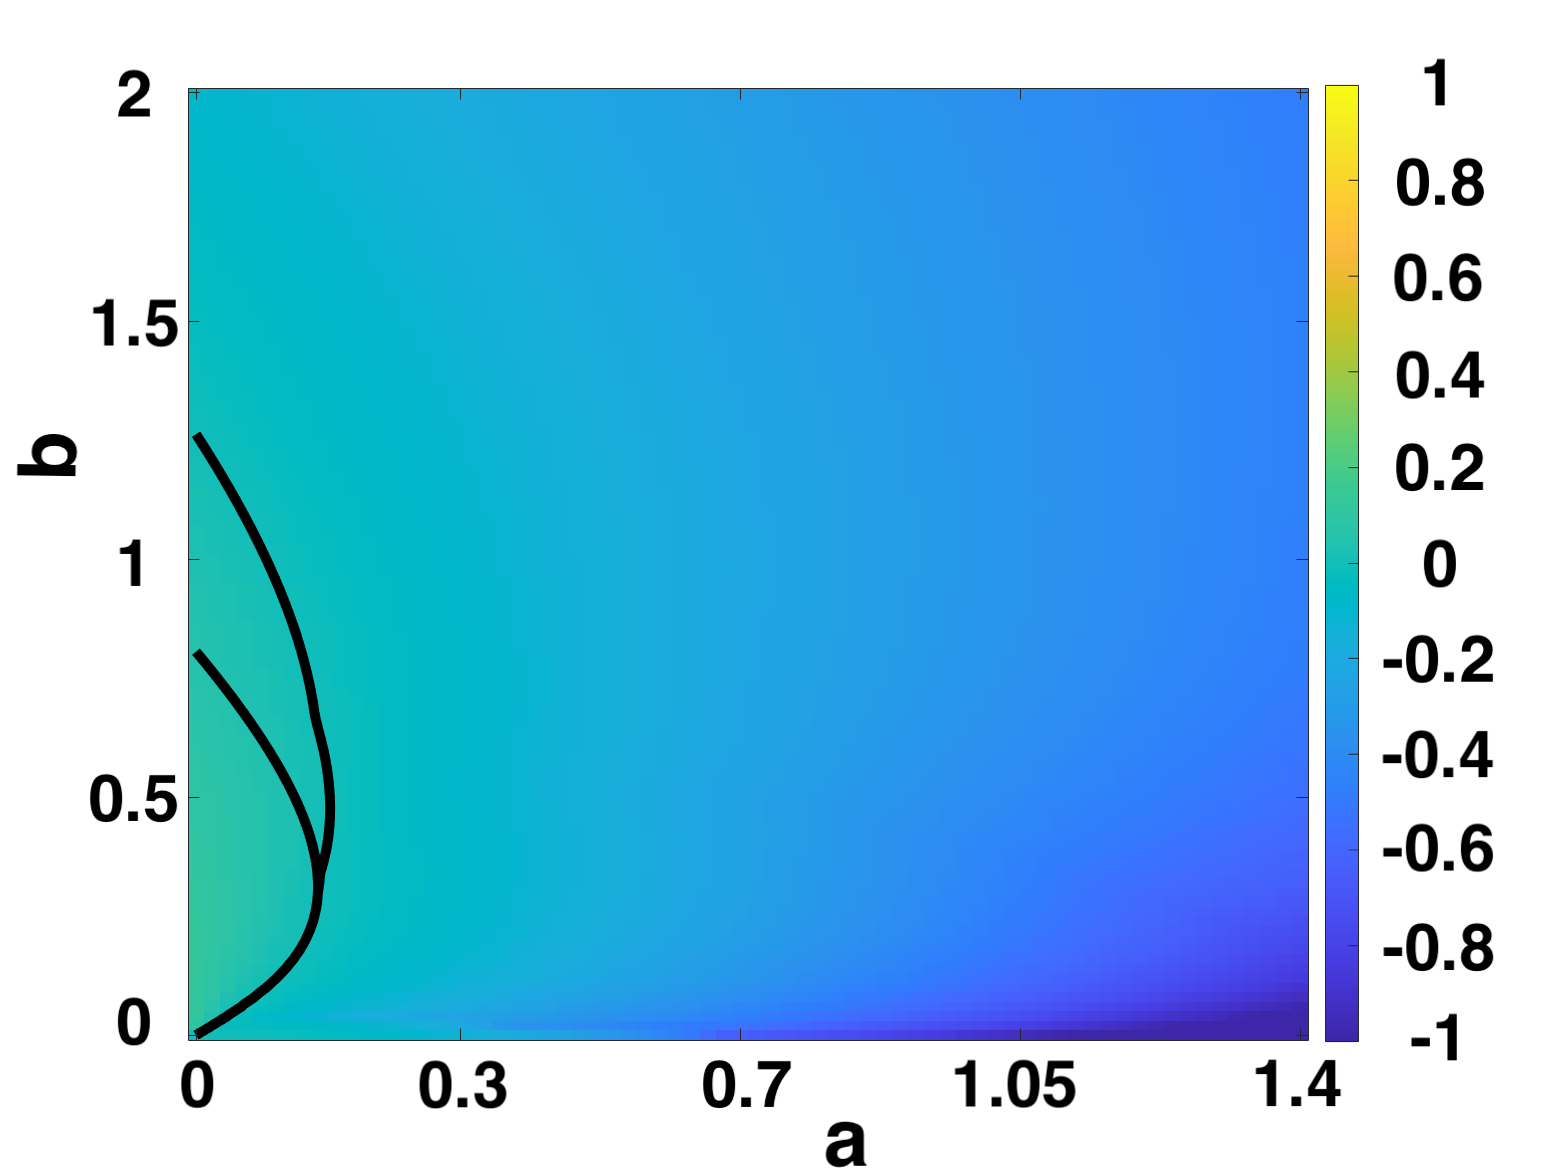
\includegraphics[width=7cm,height=5cm]{fixbif23.png}
        \caption{$\tau=1$}
        \label{}
    \end{subfigure}
    \hfill
    \begin{subfigure}[b]{0.45\textwidth}
        \centering
        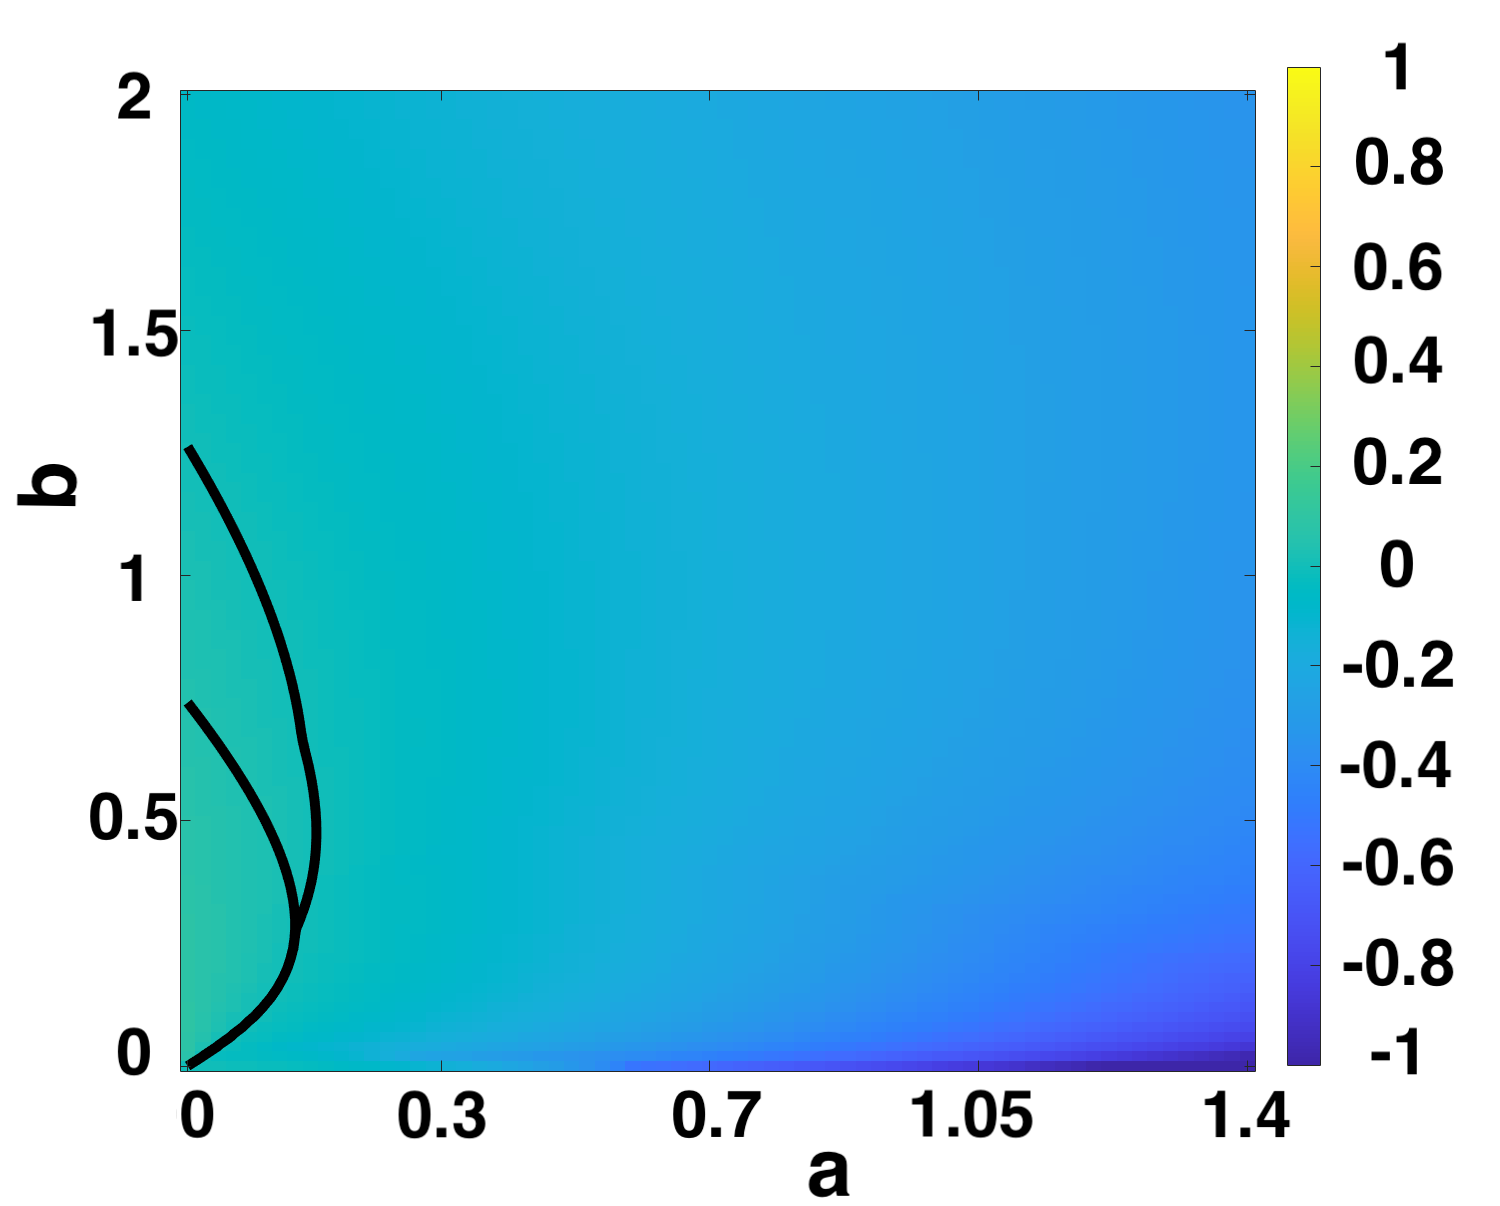
\includegraphics[width=7cm,height=5cm]{fixbif24.png}
        \caption{$\tau=1.5$.}
        \label{}
    \end{subfigure}
    \caption{$\max_k(\Re(\lambda_k))$ computed over $(a,b)$ parameter space by solving characteristic equation \eqref{characfix}, with $\epsilon^2=0.1$, $L=30\sqrt{0.05}$. As $\tau$ increases, $|\max_k(\Re(\lambda_k))|$ decreases. Contour lines for $\Re(\lambda_0)=0$ and $\max_k(\Re(\lambda))=0$ overlayed, indicated Turing instability region.}
    \label{fig:fixbif2}
\end{figure}
\section{Investigation of Variation in Initial and Boundary Conditions}
In this section, the robustness of the results obtained in \cite{gaffmonk} are examined under varying of initial conditions and boundary conditions. We first consider the sensitivity of pattern formation in the context of fixed time delay to varying initial conditions. Three different sets of initial conditions are considered. $\text{IC}_1$ corresponds to the initial conditions used in \cite{gaffmonk}. The functional form of $\text{IC}_1$ can be found in appendix (APPENDIX). The following are the forms of the remaining initial conditions used

\begin{align}
\text{IC}_2&:\quad\quad\quad\begin{pmatrix}u_0\\v_0\end{pmatrix}=\begin{pmatrix}u_\star(1+r)\\v_\star(1+r)\end{pmatrix}\quad r\sim\mathcal{N}(0,0.01)\\
\text{IC}_3&:\quad\quad\quad\begin{pmatrix}u_0\\v_0\end{pmatrix}=\begin{pmatrix}u_\star(1+r)\\v_\star(1+r)\end{pmatrix}\quad r\sim\mathcal{N}(0,0.1).
\end{align}
The model parameters used match those used in \cite{gaffmonk}, with $(a,b)=(0.1,0.9)$, and a constant history function equal to the initial conditions was used. The results in figures \ref{fig:figtau0}, \ref{fig:figtau1}, \ref{fig:figtau2}, \ref{fig:figtau4}, and \ref{fig:figtau8} show the pattern formation observed for each of the initial conditions for varying fixed time delay $\tau\in\{0,1,2,4,8 \}$.

\begin{figure}[H]
    \centering
    \begin{subfigure}[b]{0.32\textwidth}
        \centering
        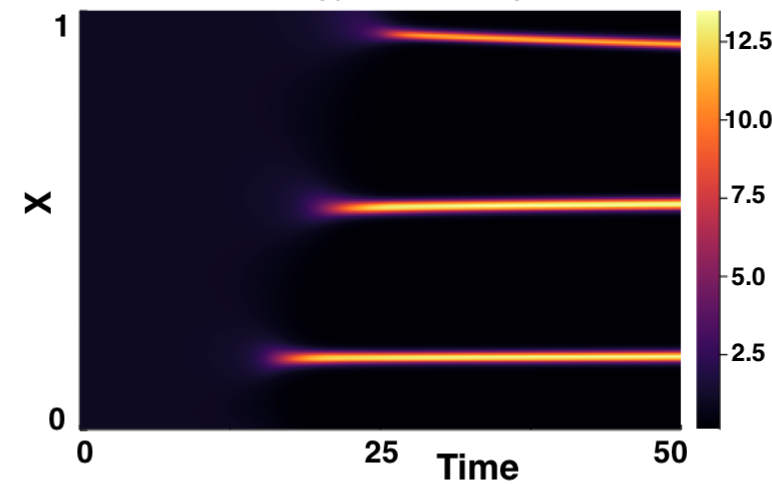
\includegraphics[width=5cm,height=4.5cm]{gaff0.png}
        \caption{$\text{IC}_1$}
        \label{}
    \end{subfigure}
    \hfill
    \begin{subfigure}[b]{0.32\textwidth}
        \centering
        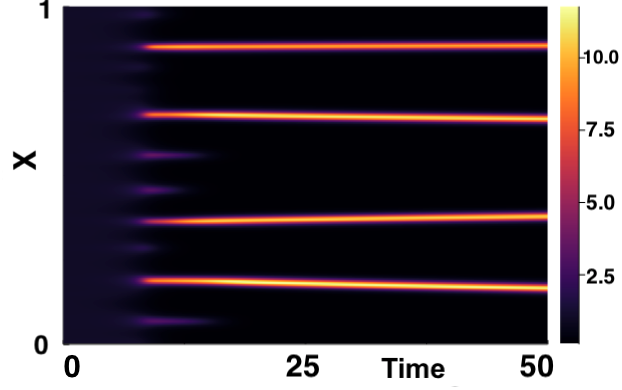
\includegraphics[width=5cm,height=4.5cm]{ic20.png}
        \caption{$\text{IC}_2$}
        \label{}
    \end{subfigure}
    \hfill
    \begin{subfigure}[b]{0.32\textwidth}
        \centering
        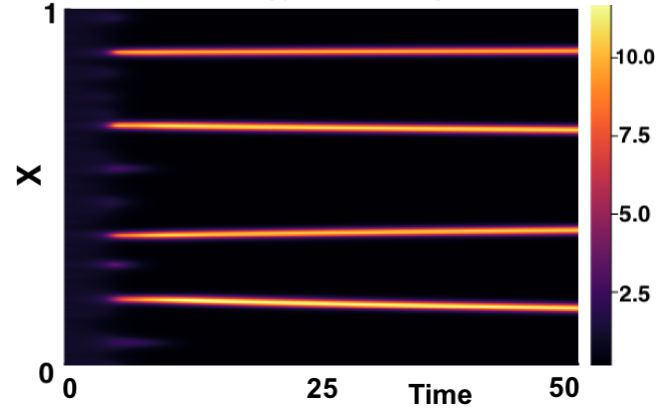
\includegraphics[width=5cm,height=4.5cm]{ic30.png}
        \caption{$\text{IC}_3$}
        \label{}
    \end{subfigure}
    \caption{Comparison of varying ICs for $\tau=0$. $(a,b)=(0.1,0.9)$, $\epsilon^2=0.001$, $L=30\sqrt{0.05}$.}
    \label{fig:figtau0}
\end{figure}
\begin{figure}[H]
    \centering
    \begin{subfigure}[b]{0.32\textwidth}
        \centering
        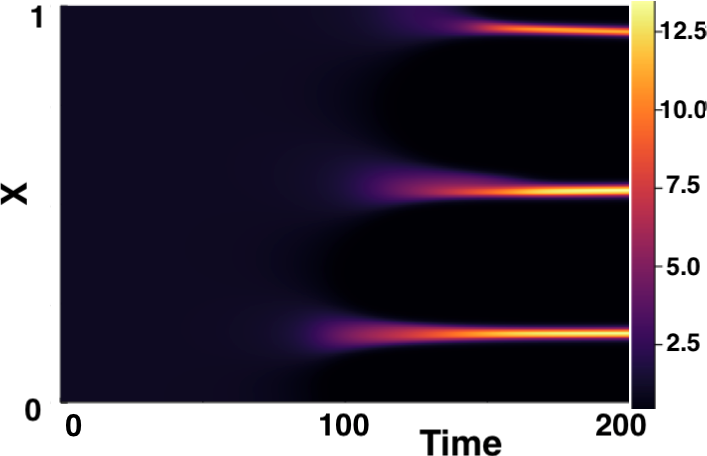
\includegraphics[width=5cm,height=4.5cm]{gaff1.png}
        \caption{$\text{IC}_1$}
        \label{}
    \end{subfigure}
    \hfill
    \begin{subfigure}[b]{0.32\textwidth}
        \centering
        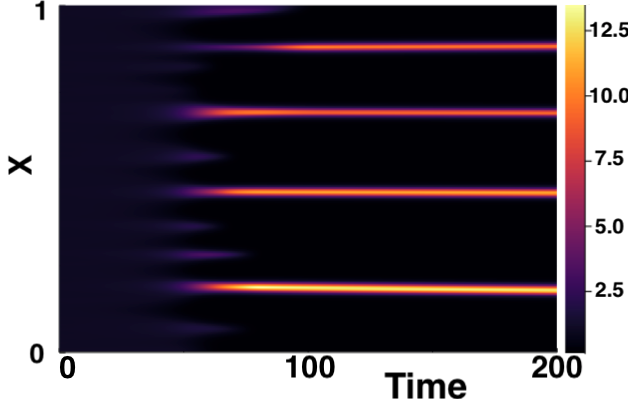
\includegraphics[width=5cm,height=4.5cm]{ic21.png}
        \caption{$\text{IC}_2$}
        \label{}
    \end{subfigure}
    \hfill
    \begin{subfigure}[b]{0.32\textwidth}
        \centering
        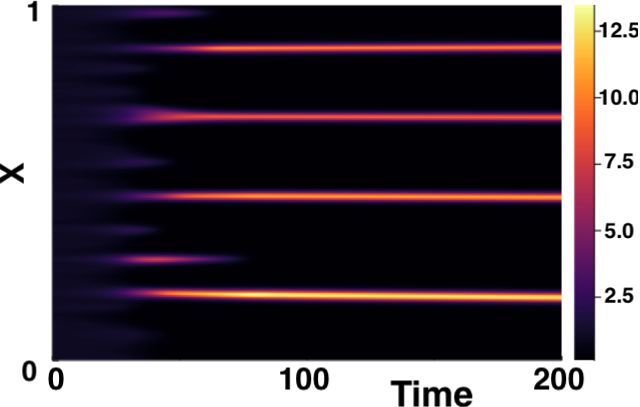
\includegraphics[width=5cm,height=4.5cm]{ic31.png}
        \caption{$\text{IC}_3$}
        \label{}
    \end{subfigure}
    \caption{Comparison of varying ICs for $\tau=1$. $(a,b)=(0.1,0.9)$, $\epsilon^2=0.001$, $L=30\sqrt{0.05}$.}
    \label{fig:figtau1}
\end{figure}
\begin{figure}[H]
    \centering
    \begin{subfigure}[b]{0.32\textwidth}
        \centering
        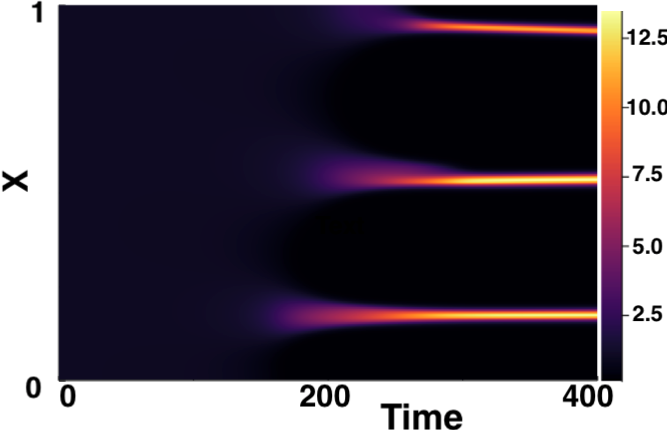
\includegraphics[width=5cm,height=4.5cm]{gaff2.png}
        \caption{$\text{IC}_1$}
        \label{}
    \end{subfigure}
    \hfill
    \begin{subfigure}[b]{0.32\textwidth}
        \centering
        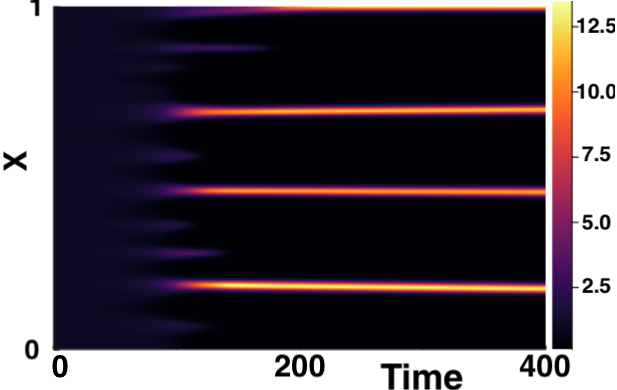
\includegraphics[width=5cm,height=4.5cm]{ic22.png}
        \caption{$\text{IC}_2$}
        \label{}
    \end{subfigure}
    \hfill
    \begin{subfigure}[b]{0.32\textwidth}
        \centering
        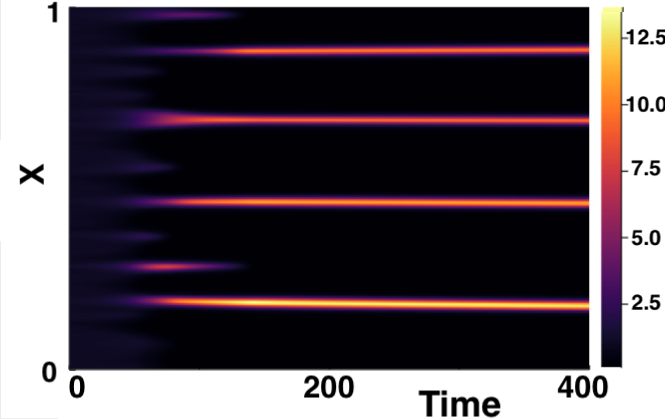
\includegraphics[width=5cm,height=4.5cm]{ic32.png}
        \caption{$\text{IC}_3$}
        \label{}
    \end{subfigure}
    \caption{Comparison of varying ICs for $\tau=2$. $(a,b)=(0.1,0.9)$, $\epsilon^2=0.001$, $L=30\sqrt{0.05}$.}
    \label{fig:figtau2}
\end{figure}
\begin{figure}[H]
    \centering
    \begin{subfigure}[b]{0.32\textwidth}
        \centering
        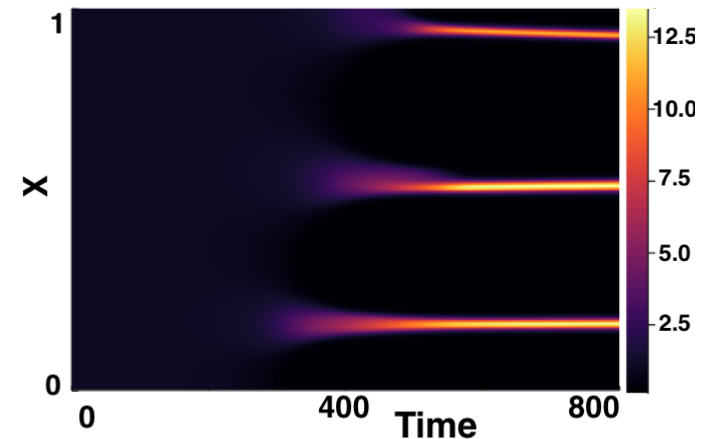
\includegraphics[width=5cm,height=4.5cm]{gaff4.png}
        \caption{$\text{IC}_1$}
        \label{}
    \end{subfigure}
    \hfill
    \begin{subfigure}[b]{0.32\textwidth}
        \centering
        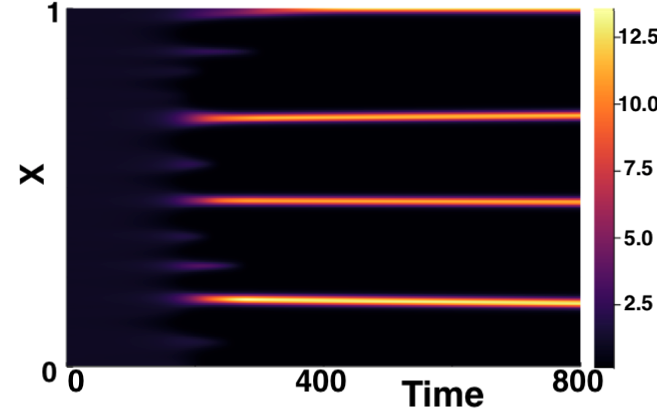
\includegraphics[width=5cm,height=4.5cm]{ic24.png}
        \caption{$\text{IC}_2$}
        \label{}
    \end{subfigure}
    \hfill
    \begin{subfigure}[b]{0.32\textwidth}
        \centering
        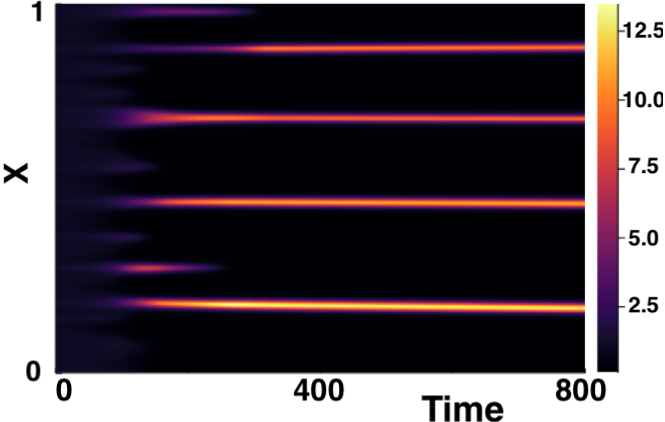
\includegraphics[width=5cm,height=4.5cm]{ic34.png}
        \caption{$\text{IC}_3$}
        \label{}
    \end{subfigure}
    \caption{Comparison of varying ICs for $\tau=4$. $(a,b)=(0.1,0.9)$, $\epsilon^2=0.001$, $L=30\sqrt{0.05}$.}
    \label{fig:figtau4}
\end{figure}
\begin{figure}[H]
    \centering
    \begin{subfigure}[b]{0.32\textwidth}
        \centering
        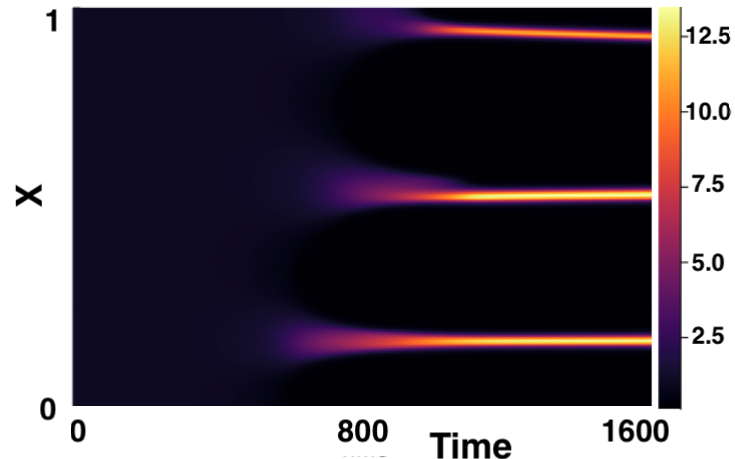
\includegraphics[width=5cm,height=4.5cm]{gaff8.png}
        \caption{$\text{IC}_1$}
        \label{}
    \end{subfigure}
    \hfill
    \begin{subfigure}[b]{0.32\textwidth}
        \centering
        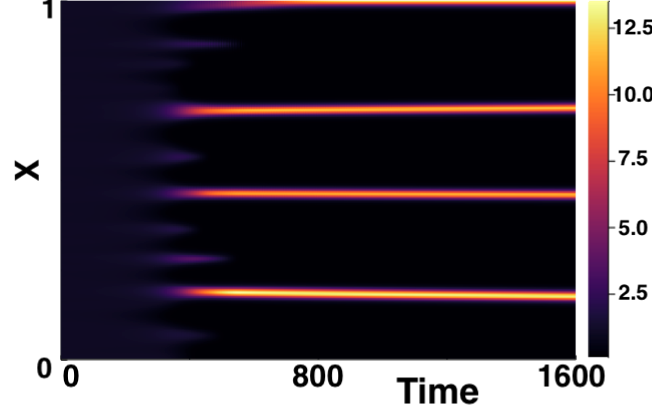
\includegraphics[width=5cm,height=4.5cm]{ic28.png}
        \caption{$\text{IC}_2$}
        \label{}
    \end{subfigure}
    \hfill
    \begin{subfigure}[b]{0.32\textwidth}
        \centering
        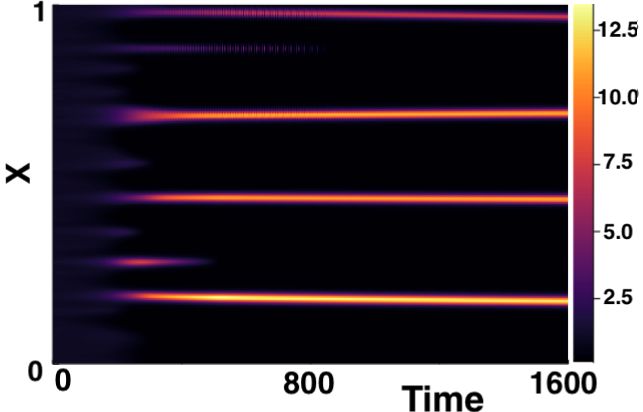
\includegraphics[width=5cm,height=4.5cm]{ic38.png}
        \caption{$\text{IC}_3$}
        \label{}
    \end{subfigure}
    \caption{Comparison of varying ICs for $\tau=8$. $(a,b)=(0.1,0.9)$, $\epsilon^2=0.001$, $L=30\sqrt{0.05}$.}
    \label{fig:figtau8}
\end{figure}

It can be seen that the choice of initial conditions when considering the effect of time delay on Turing pattern formation is extremely important. The choice of a random Gaussian perturbation rather than the functional form given in $\text{IC}_1$ also results in four `spikes' in the solution, rather than three. We also observe, for all initial conditions used, an approximate linear relationship between $\tau$ and the time taken for pattern formation to occur. As $\tau$ is doubled the time taken for the pattern to form is appears to double. This can be seen clearly by considering figures in the same column and considering the point where spikes can first be seen along the $x$ axis. This is a relationship that is further explored in section \ref{section:delaypatt}.
\\\\
Numerical results were also simulated to study the effects of a temporal variation in the history function. A history function was set as $h(t)=u_\star(1+r\sin(\omega t))$ for $t\in[-\tau,0)$, where $r$ is the random variable used in $\text{IC}_2$. Simulations were conducted for varying $\tau$ and $\omega$. Preliminary simulations, which can be found in appendix (APPENDIX), show that this type of variation in history does not have a significant effect on the results seen.
\\\\
Finally, we consider the effect of varying boundary conditions. Motivated from the analysis in \cite{krausemixed}, homogeneous Dirichlet boundary conditions are implemented for the activator term, and homogeneous Neumann boundary conditions implemented for the inhibitor term. Thus, we have that, on a domain $\Omega=[0,1]$, $u=0$ and $\frac{\partial v}{\partial t}=0$ at $x=0, 1$. These conditions are implemented numerically following the methodology outlined in section \ref{section:numimp}. The results in figures \ref{fig:bctau1}, \ref{fig:bctau2}, and \ref{fig:bctau3} were generated using $\text{IC}_2$, with a varying $\tau\in\{0,1,2\}$, and show the comparison between numerical simulations generated with homogeneous Neumann conditions for both $u$ and $v$, indicated as $\text{BC}_1$, and those generated with homogeneous Dirichlet conditions for $u$, indicated as $\text{BC}_2$.

\begin{figure}[H]
    \centering
    \begin{subfigure}[b]{0.45\textwidth}
        \centering
        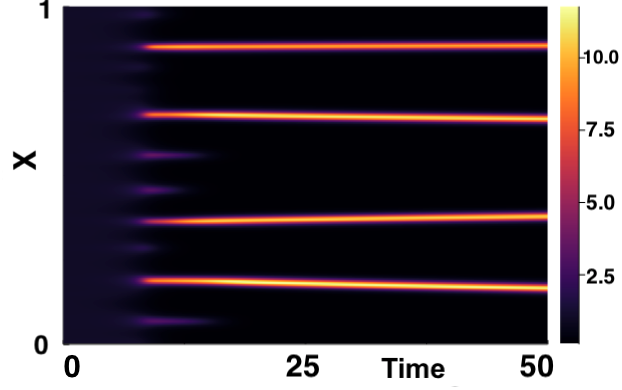
\includegraphics[width=7cm,height=5.5cm]{ic20.png}
        \caption{$\text{BC}_1$}
        \label{}
    \end{subfigure}
    \hfill
    \begin{subfigure}[b]{0.45\textwidth}
        \centering
        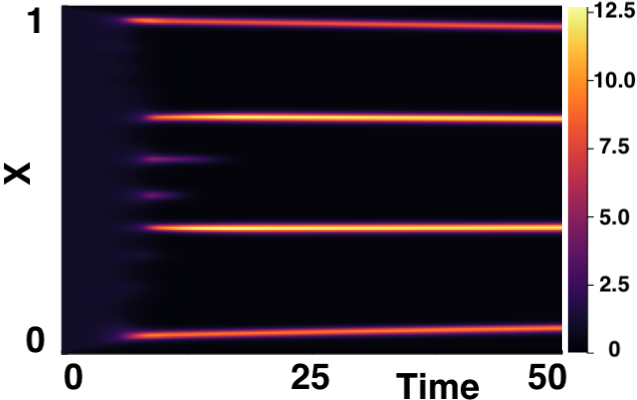
\includegraphics[width=7cm,height=5.5cm]{bc0.png}
        \caption{$\text{BC}_2$}
        \label{}
    \end{subfigure}
    \caption{Comparison of varying BCs for $\tau=0$. Generated with $\text{IC}_2$. $(a,b)=(0.1,0.9)$, $\epsilon^2=0.001$, $L=30\sqrt{0.05}$.}
    \label{fig:bctau1}
\end{figure}

\begin{figure}[H]
    \centering
    \begin{subfigure}[b]{0.45\textwidth}
        \centering
        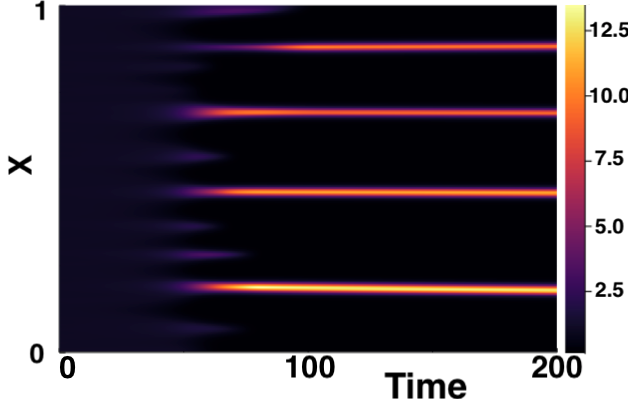
\includegraphics[width=7cm,height=5.5cm]{ic21.png}
        \caption{$\text{BC}_1$}
        \label{}
    \end{subfigure}
    \hfill
    \begin{subfigure}[b]{0.45\textwidth}
        \centering
        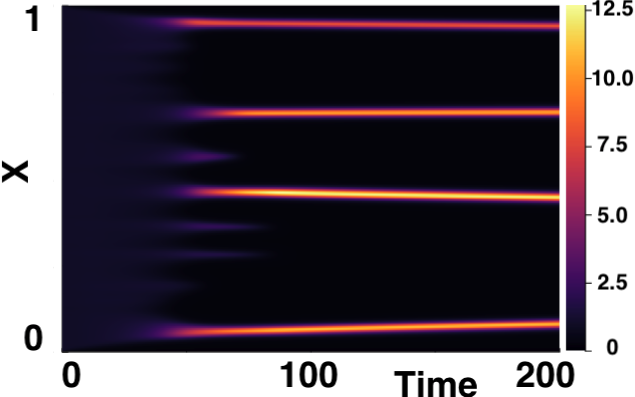
\includegraphics[width=7cm,height=5.5cm]{bc1.png}
        \caption{$\text{BC}_2$}
        \label{}
    \end{subfigure}
    \caption{Comparison of varying BCs for $\tau=1$. Generated with $\text{IC}_2$. $(a,b)=(0.1,0.9)$, $\epsilon^2=0.001$, $L=30\sqrt{0.05}$.}
    \label{fig:bctau2}
\end{figure}

\begin{figure}[H]
    \centering
    \begin{subfigure}[b]{0.45\textwidth}
        \centering
        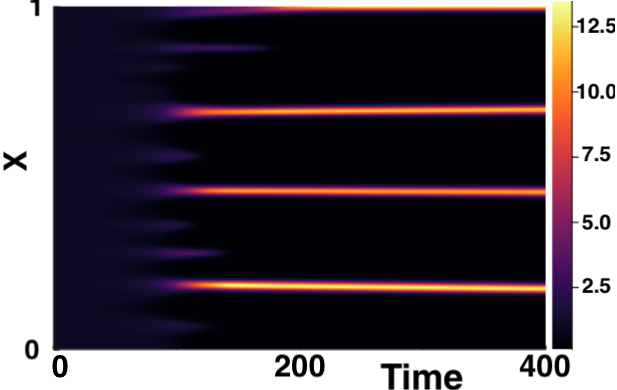
\includegraphics[width=7cm,height=5.5cm]{ic22.png}
        \caption{$\text{BC}_1$}
        \label{}
    \end{subfigure}
    \hfill
    \begin{subfigure}[b]{0.45\textwidth}
        \centering
        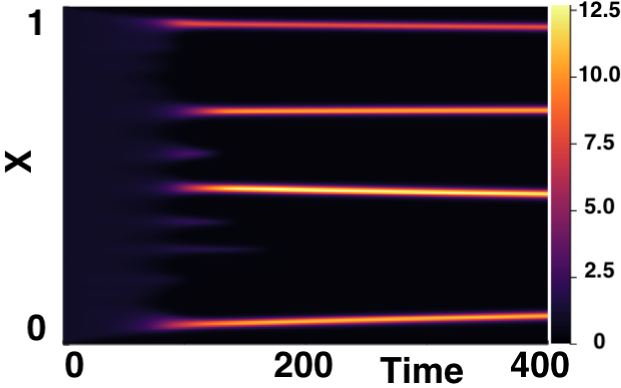
\includegraphics[width=7cm,height=5.5cm]{bc2.png}
        \caption{$\text{BC}_2$}
        \label{}
    \end{subfigure}
    \caption{Comparison of varying BCs for $\tau=2$. Generated with $\text{IC}_2$. $(a,b)=(0.1,0.9)$, $\epsilon^2=0.001$, $L=30\sqrt{0.05}$.}
    \label{fig:bctau3}
\end{figure}

\section{Relationship Between Time-To-Pattern and time delay}\label{section:delaypatt}

We aim to show that, for small $\tau$ and small $L$, the linear theory provides a good approximation to the time taken until pattern formation occurs, and in fact, the relationship between $\tau$ and time-to-pattern under these conditions is linear. We also show that, through full numerical solutions, the relationship between $\tau$ and time-to-pattern on a longer time-scale for larger $\tau$ is also linear. We first consider the former.
\\\\
To minimise the effect of nonlinearity in the dynamics, we restrict the domain size to $L=2\sqrt{0.05}$. Shrinking the domain results in fewer unstable modes and thus less competition for the dominant mode, resulting in a better approximation of the linear theory. This finite size effect can be seen in figure \ref{fig:compardisp}, where $\Re(\lambda_k)$ is plotted against $k$ for two different domain sizes, for a given $(a,b,\tau)$. Due to numerical restrictions when using Chebfun in finding roots of the characteristic equation \eqref{characfix}, only $\tau\leq1.6$ is considered. Similar to the initial conditions used for previous numerical simulations (figure \ref{fig:fixedsim2}), we take a small perturbation in the activator term, $\hat{u}(t)$, such that $\hat{u}(0)=ru_\star$, where $r$ is a small Gaussian random variable, $r\sim\mathcal{N}(0,\sigma^2)$,
for some standard deviation $\sigma$.
\\\\
The linear theory suggests that at some time $t=T$, the perturbation will be of the form $\hat{u}(T)\sim A_k(T)\cos(k\pi x)$, where $k$ is the dominant mode and $A_k(T)$ denotes the corresponding Fourier coefficient at time $t=T$. For a given parameter set $(a,b,\epsilon^2,\tau,L)$, we can solve the characteristic equation \eqref{characfix}, and plot $\Re(\lambda_k)$
against $k$, to determine the dominating mode $k$ and the corresponding eigenvalue, or growth rate, $\lambda_k$. We then use this information in the following manner: A Fast Fourier Transform to decompose the initial conditions into a Fourier series is used, and the coefficient $A_k(0)$ for the dominating $k$ is computed. When the perturbation $\hat{u}$ has grown sufficiently, in absolute value, beyond a threshold where pattern formation is considered, we call this time $t=T$, and again determine the Fourier coefficient $A_k(T)$ of the fastest-growing mode $k$. More specifically, the time $T$ is such that $\max_x|u(T,x)-u_\star|>\text{threshold}$, namely the first time such that any solution point across the whole spatial domain is large enough, in absolute difference, from the steady-state.
\\\\
Using the relation $A_k(T)\sim A_k(0)e^{\lambda_k T}$, we rearrange for $T$ and thus compute a linear approximation for time-to-pattern as
\begin{equation}
    T=\frac{1}{\lambda_k}\ln\left(\frac{A_k(T)}{A_k(0)}\right).
\end{equation}
The standard deviation for the random variable $r$ is given as $\sigma=10^{-5}$, and the threshold value at $0.1$. A very small perturbation was used as a means to improve the accuracy of the linear theory.
\begin{figure}[H]
    \centering
    \begin{subfigure}[b]{0.45\textwidth}
        \centering
        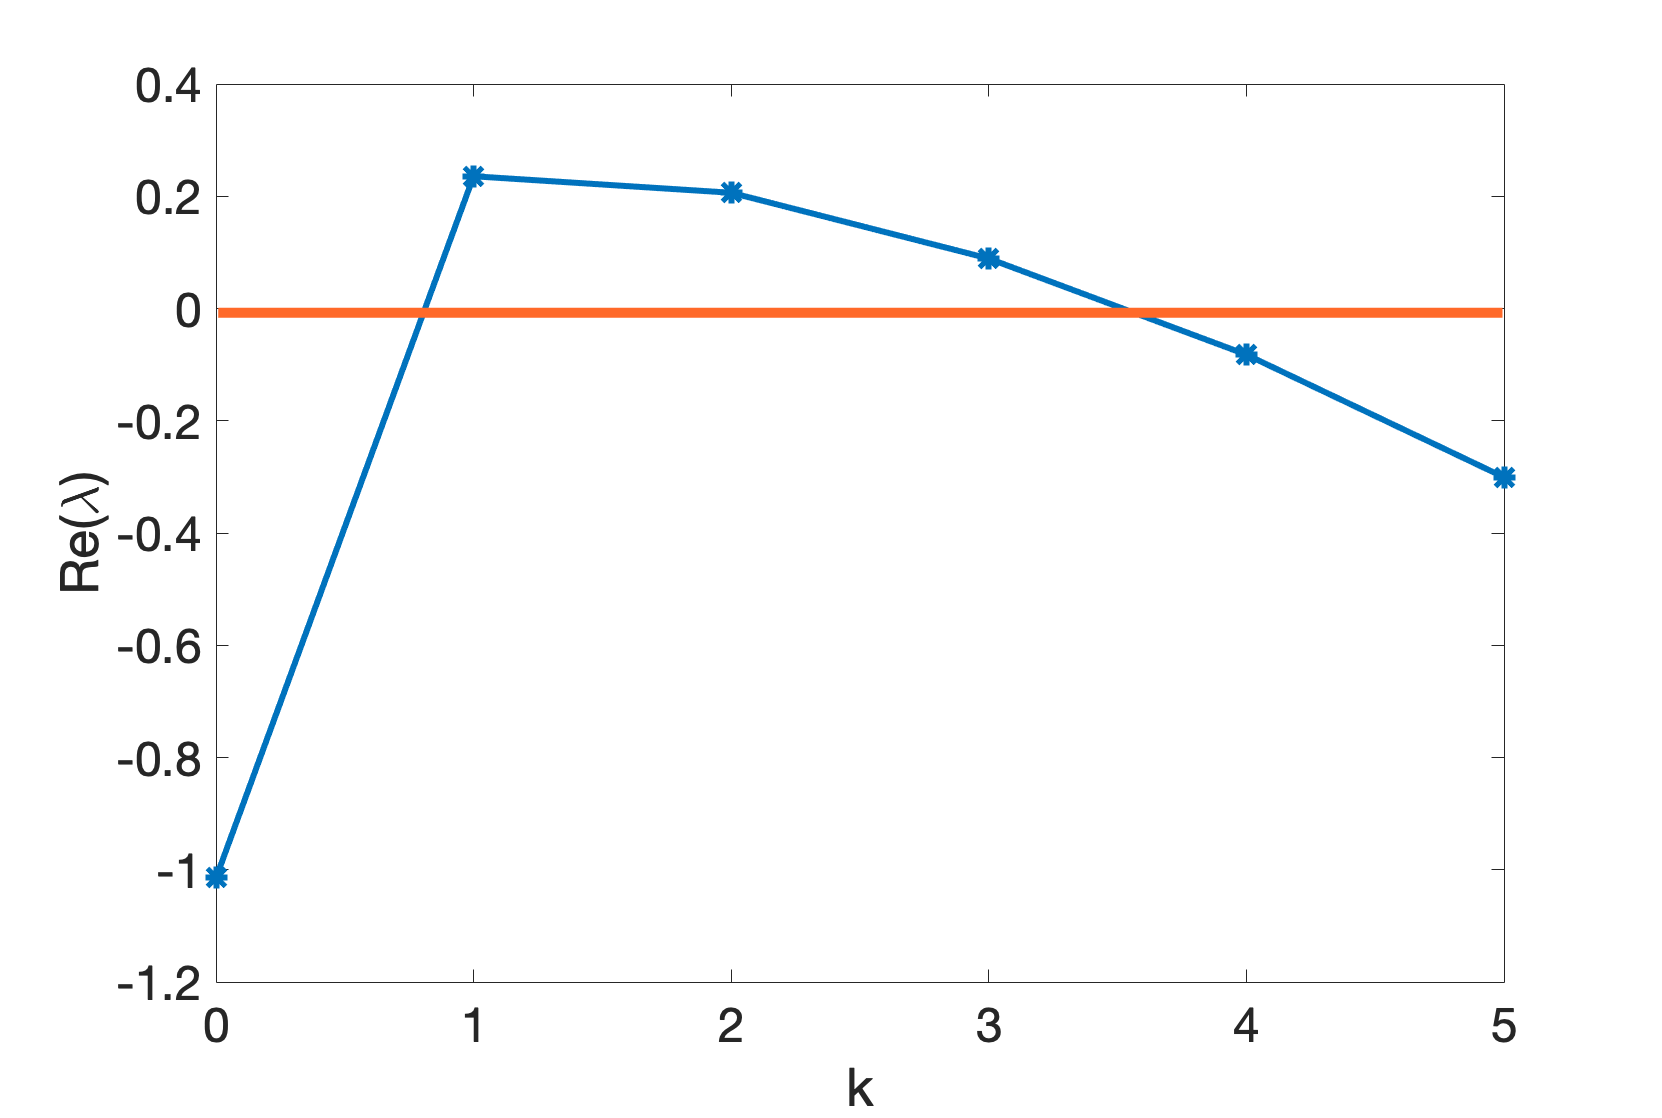
\includegraphics[width=7cm,height=5.5cm]{compdisp1.png}
        \caption{Dispersion curve plotted with domain size $L=2\sqrt{0.05}$.}
        \label{fig:compdisp1}
    \end{subfigure}
    \hfill
    \begin{subfigure}[b]{0.45\textwidth}
        \centering
        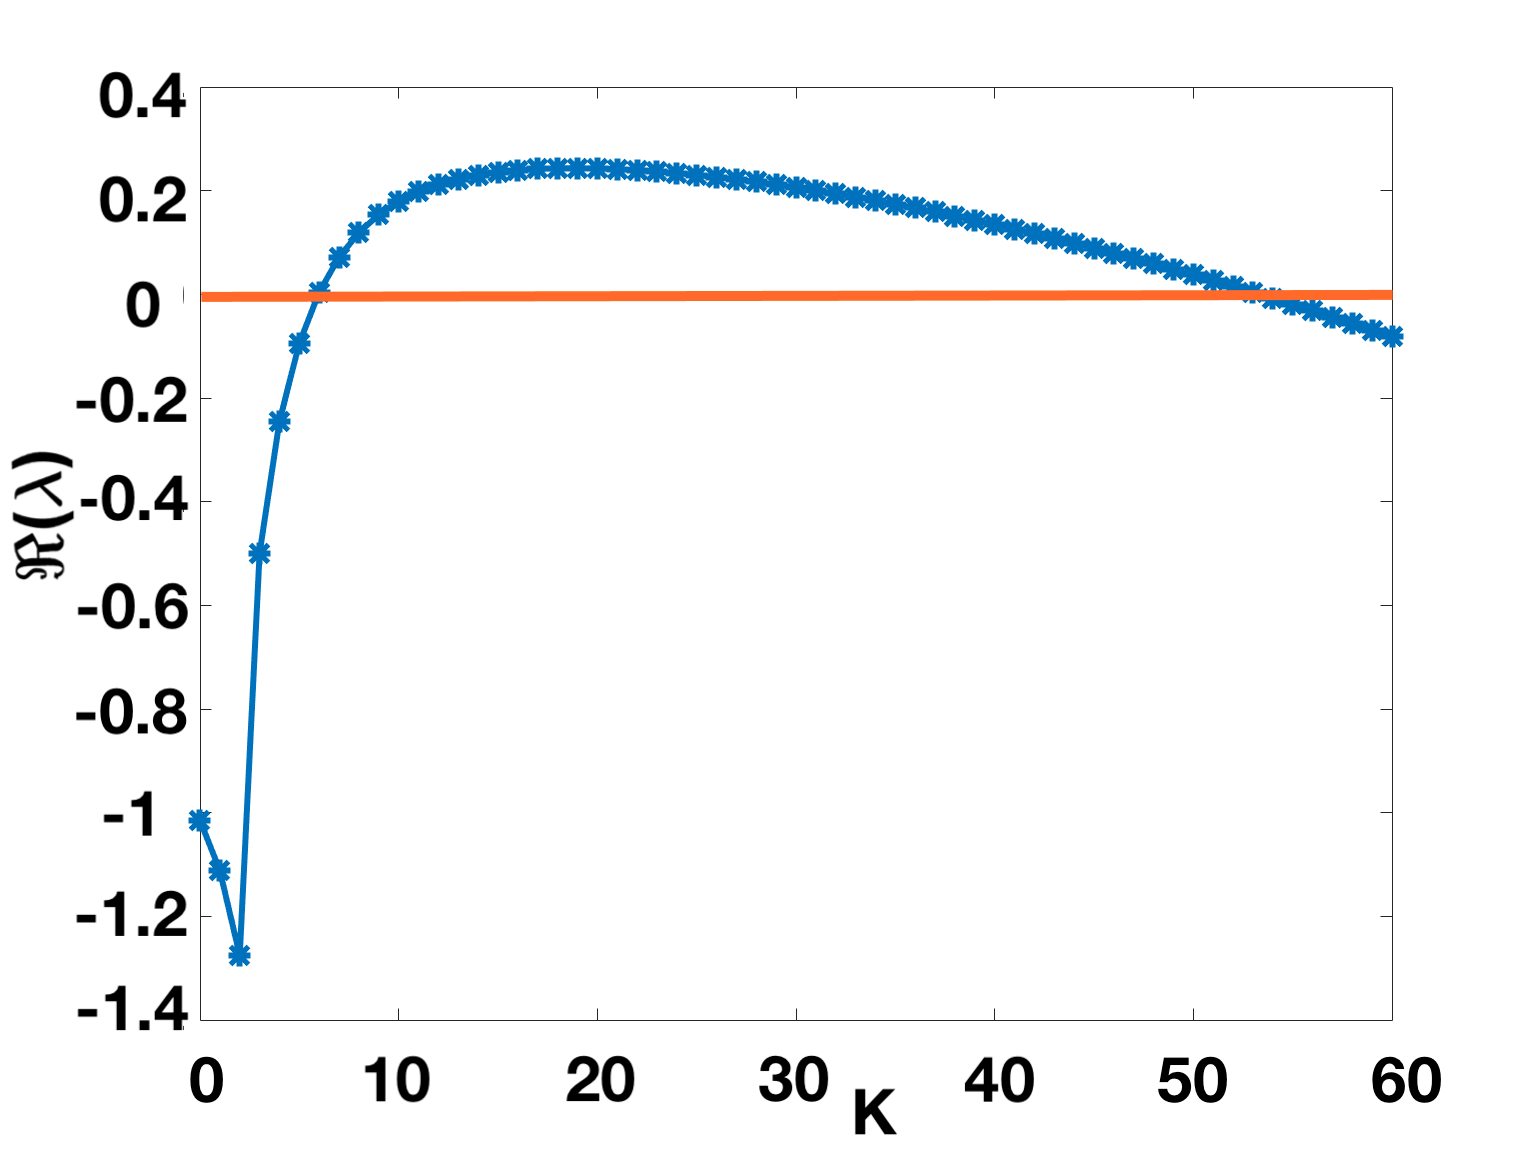
\includegraphics[width=7cm,height=5.5cm]{compdisp2.png}
        \caption{Dispersion curve plotted with domain size $L=30\sqrt{0.05}$.}
        \label{fig:compdisp2}
    \end{subfigure}
    \caption{Dispersion curves plotted for $(a,b,\tau)=(0.4,1.8,0.2)$ and $\epsilon^2=0.001$. A larger $L$ results in more unstable modes $\lambda_k$ such that $\Re(\lambda)>0$. }
    \label{fig:compardisp}
\end{figure}
Using $\epsilon^2=0.001$, on the domain size $L=2\sqrt{0.05}$, figure \ref{fig:compdisp1} suggests that at $\tau=0.2$, from the linear theory, the dominant mode is $k=1$ with dominant eigenvalue $\lambda_1=0.2356$. Figure \ref{fig:icfc} shows the initial condition used, with random perturbation $\hat{u}(0)=ru_\star$, and the plotted Fourier coefficients $A_k(0)$, in absolute value, for $k\neq0$.
\begin{figure}[H]
    \centering
    \begin{subfigure}[b]{0.45\textwidth}
        \centering
        \includegraphics[width=7cm,height=6cm]{uic.png}
        \caption{Initial conditions of activator $u$ across spatial domain.}
        \label{}
    \end{subfigure}
    \hfill
    \begin{subfigure}[b]{0.45\textwidth}
        \centering
        \includegraphics[width=7cm,height=6cm]{uicfc.png}
        \caption{Absolute Fourier coefficients, $|A_k(0)|$, of initial conditions, $k\neq0$.}
        \label{fig:}
    \end{subfigure}
    \caption{Initial conditions as a small Gaussian perturbation of $O(10^{-5})$. Fourier coefficients $A_k(0)$ computed using Fast Fourier Transform. Parameter values are $(a,b)=(0.4,1.8)$.}
    \label{fig:icfc}
\end{figure}
Since $k=1$ is the dominant mode, we extract the first Fourier coefficient of the initial conditions, $A_1(0)$, as $A_1(0)=7.95(3.s.f)\times10^{-8}$. To find $A_1(T)$, a numerical simulation is run until the perturbation of $O(10^{-5})$ has grown, in absolute value, to a threshold value of $0.1$. Simulating first for a time delay $\tau=0.2$, figure \ref{fig:Tfc} shows the numerical solution $u(T)$ at the point where the perturbation has grown to this threshold value, as well as a scatter plot of the Fourier coefficients $A_k(T)$, $k\neq0$.
\begin{figure}[H]
    \centering
    \begin{subfigure}[b]{0.45\textwidth}
        \centering
        \includegraphics[width=7cm,height=6cm]{Tu.png}
        \caption{Numerical solution $u(T)$ at $t=T$}
        \label{uT}
    \end{subfigure}
    \hfill
    \begin{subfigure}[b]{0.45\textwidth}
        \centering
        \includegraphics[width=7cm,height=6cm]{Tfc.png}
        \caption{Absolute Fourier coefficients of $u(T)$.}
        \label{fig:uTfc}
    \end{subfigure}
    \caption{Numerical solution and Fourier coefficients for $u(T)$, with $(a,b)=(0.4,1.8)$, time delay $\tau=0.2$ and $\epsilon^2=0.002$, $L=2\sqrt{0.05}$.}
    \label{fig:Tfc}
\end{figure}
As seen in figure \ref{fig:uTfc}, the Fourier coefficient corresponding to $k=1$ is given as $0.0262(3.s.f)$. The approximated time-to-pattern, as predicted by linear theory, for $(a,b,\tau)=(0.4,1.8,0.2)$ and the given initial conditions is thus computed as
\begin{equation}
    T=\frac{1}{\lambda_1}\ln\left(\frac{A_1(T)}{A_1(0)}\right)=\frac{1}{0.2356}\ln\left(\frac{0.0262}{7.95\times10^{-8}}\right)=53.8(3.s.f).
\end{equation}
It was found through numerical solutions that the `true' time-to-pattern is $\approx57.5(3sf)$.
We use `true' time-to-pattern here to mean the time taken for a perturbation to grow above a threshold value found through full numerical solutions.
 The numerical solution of $(a,b,\tau)=(0.4,0.8,0.2)$ with $L=2\sqrt{0.05}$ and $\epsilon^2=0.001$, for a timespan $t\in[0,100]$ can be seen in figure \ref{fig:dispnumsim}. The process above can be repeated for varying $(a,b,\tau)$, and figures \ref{fig:ttp1}, \ref{fig:ttp2}, \ref{fig:ttp3} show the predicted time-to-pattern plotted against $\tau$ and compared with the `true' time-to-pattern for three different parameter sets. The time delay is varied here over $\tau\in[0,1.6]$ at intervals of $0.2$.

\begin{figure}[H]
    \centering
    \begin{subfigure}[b]{0.45\textwidth}
        \centering
        \includegraphics[width=7cm,height=6cm]{dispnumsim.png}
        \caption{Numerical solution for $(a,b,\tau)=(0.4,1.8,0.2)$, $L=2\sqrt{0.05}$, $\epsilon^2=0.001$.}
        \label{fig:dispnumsim}
    \end{subfigure}
    \hfill
    \begin{subfigure}[b]{0.45\textwidth}
        \centering
        \includegraphics[width=7cm,height=6cm]{ttp1.png}
        \caption{Predicted vs `true' time-to-pattern for $(a,b)=(0.4,1.8)$, $L=2\sqrt{0.05}$, $\epsilon^2=0.001$, and $\tau\in[0,1.6]$.}
        \label{fig:ttp1}
    \end{subfigure}
    \caption{}
    \label{}
\end{figure}

\begin{figure}[H]
    \centering
    \begin{subfigure}[b]{0.45\textwidth}
        \centering
        \includegraphics[width=7cm,height=6cm]{ttp2.png}
        \caption{Predicted vs `true' time-to-pattern for $(a,b)=(0.1,0.9)$, $L=2\sqrt{0.05}$, $\epsilon^2=0.001$, and $\tau\in[0,1.6]$.}
        \label{fig:ttp2}
    \end{subfigure}
    \hfill
    \begin{subfigure}[b]{0.45\textwidth}
        \centering
        \includegraphics[width=7cm,height=6cm]{ttp3.png}
        \caption{Predicted vs `true' time-to-pattern for $(a,b)=(0.2,1.3)$, $L=2\sqrt{0.05}$, $\epsilon^2=0.001$, and $\tau\in[0,1.6]$.}
        \label{fig:ttp3}
    \end{subfigure}
    \caption{}
    \label{}
\end{figure}

Now, through full numerical solutions, we show a linear relationship between $\tau$ and time-to-pattern on a longer time-scale. Varying $\tau\in[1,16]$ at regular intervals of $1$, for two different parameter sets $(a,b)=\{(0.1,0.9),(0.4,0.8)\}$, we compute the time taken for a perturbation to grow up to a threshold value, and plot the results. Figure \ref{fig:linperturb1a} shows the results for $(a,b)=(0.1,0.9)$ with an initial perturbation of standard-deviation $\sigma=10^{-5}$ and threshold value $0.1$. Figure \ref{fig:linperturb1b} shows the results for the same parameter values but with an initial perturbation of standard-deviation $\sigma=0.01$ and threshold value $2$. Figures \ref{fig:linperturb2a} and \ref{fig:linperturb2b} show analogous results but for $(a,b)=(0.4,0.8)$. The simulations were run with $\epsilon^2=0.001$ and $L=30\sqrt{0.05}$.
\begin{figure}[H]
    \centering
    \begin{subfigure}[b]{0.45\textwidth}
        \centering
        \includegraphics[width=7cm,height=6cm]{longlin2.png}
        \caption{$(a,b)=(0.1,0.9)$ with $\sigma=10^{-5}$ and threshold $0.1$.}
        \label{fig:linperturb1a}
    \end{subfigure}
    \hfill
    \begin{subfigure}[b]{0.45\textwidth}
        \centering
        \includegraphics[width=7cm,height=6cm]{longlin1.png}
        \caption{$(a,b)=(0.1,0.9)$ with $\sigma=0.01$ and threshold $2$}
        \label{fig:linperturb1b}
    \end{subfigure}
    \caption{Time-to-pattern plotted against $\tau$ for two different initial conditions. $(a,b)=(0.1,0.9)$, $\epsilon^2=0.001$ and domain size $L=30\sqrt{0.05}$.}
    \label{}
\end{figure}

\begin{figure}[H]
    \centering
    \begin{subfigure}[b]{0.45\textwidth}
        \centering
        \includegraphics[width=7cm,height=6cm]{longlin3.png}
        \caption{$(a,b)=(0.4,0.8)$ with $\sigma=10^{-5}$ and threshold $0.1$}
        \label{fig:linperturb2a}
    \end{subfigure}
    \hfill
    \begin{subfigure}[b]{0.45\textwidth}
        \centering
        \includegraphics[width=7cm,height=6cm]{longlin4.png}
        \caption{$(a,b)=(0.4,0.8)$ with $\sigma=0.01$ and threshold $2$}
        \label{fig:linperturb2b}
    \end{subfigure}
    \caption{Time-to-pattern plotted against $\tau$ for two different initial conditions. $(a,b)=(0.4,0.8)$, $\epsilon^2=0.001$ and domain size $L=30\sqrt{0.05}$.}
    \label{}
\end{figure}


\section{Summary}

In this chapter, we presented the biological motivation for studying the LI variant of the Schnakenberg model with incorporated fixed delay.
\\\\
Linear theory suggested that for the LI model, time delay can act as a stabilising agent for Turing instabilities, increasing the parameter region where Turing instabilities can occur. Through both linear analysis on a small scale, and full numerical solutions on a larger scale, a linear relationship between time delay and time-to-pattern was presented, and an increasing delay was shown to, depending on the parameter chosen, increase the time taken for pattern formation to occur, or increase the time taken for perturbations to fully decay.
\\\\
Numerical results in this chapter were also systematically tested with a varying of initial and boundary conditions, and also a temporal variation in the history function was introduced. Simulations suggested that the increase in time-to-pattern with an increase in delay is robust to these variations. We therefore look for ways to remedy the problems caused by a fixed delay. Considering the complexity and stochastic nature of pattern formation on a cellular level leads us to consider modelling the time delay as a distrbution, which we consider in the next chapter.
